This chapter focuses on investigating the dynamic material response of epithelial domes to varying strain, tension, and pressure. In a morphogenetic context, pressure levels can vary significantly across a wide range of magnitudes and timescales in different situations \cite{torres-sanchez2021, choudhury2022a}. For example, during blastocyst development, luminal pressure doubles, leading to changes in cortical tension and cellular strain \cite{chan2019}.

In the case of epithelial domes, \citet{latorre2018} observed a broad spectrum of pressure levels throughout dome evolution, resulting in various cellular deformations and tissue behaviors including active-superelasticity. However, in this system, control is limited to the footprint of the domes, with no capability to control pressure and tension. To address this limitation, in this chapter, we will employ the monolayer inflator (MOLI) system to subject tissues to different strain and tension regimes and characterize the material response of epithelial tissues.

\hypertarget{measurement-of-dome-mechanics}{%
	\section{Measurement of dome mechanics}\label{measurement-of-dome-mechanics}}

To characterize the dynamics of the domes, we assumed that the shape of domes closely follows a spherical cap geometry, and hence we focused on the midsection (see Figure \ref{fig_7_1}). This  approximation is reasonable for domes with circular footprint. For spherical domes  supporting a membrane state of stress, mechanical equilibrium tangential to the surface implies that tension is isotropic and uniform tension, whereas mechanical equilibrium normal to the surface is expressed by Laplace's law \cite{latorre2018}. However, MOLI can also be applied to map the  heterogeneous and anisotropic tension of non-spherical domes, e.g.~resulting from non-circular footprints, applying curved Monolayer Stress Microscopy \cite{marin-llaurado2022}.

From the cross-section, we measured the height $h$ and base radius $a$ of each dome, which allowed us to calculate the radius of curvature $R$ as
\begin{equation}
	\label{eqn:radiuscurve}
	R = \frac{h^2 + a^2}{2h}.
\end{equation}
Additionally, we MOLI provides a direct readout of pressure $\Delta P$, allowing us to compute the tension ($\sigma$) using Laplace's law
\begin{equation}
	\label{eqn:laplace}
	\sigma = \frac{\Delta PR }{2} .
\end{equation}

To quantify dome deformation, we used the areal strain measure, which is defined as the difference between the dome surface area ($A$) and the area of the footprint ($A_{0}$) normalized by the latter, leading to
\begin{equation}
	\label{eqn:arealstrain}
	\epsilon = \frac{A - A_{0}}{A_{0}} = \frac{\pi(h^2 + a^2) - \pi a^2}{\pi a^2} = \frac{h^2}{a^2} .
\end{equation}
To obtain the temporal evolution of the dome’s geometry, we generated kymographs of the top section of the domes. These kymographs provide the time evolution of $h$. Given $a$ and the applied pressure as a function of time, we computed tensions and strain using the relations above.

\begin{figure}
	\centering
	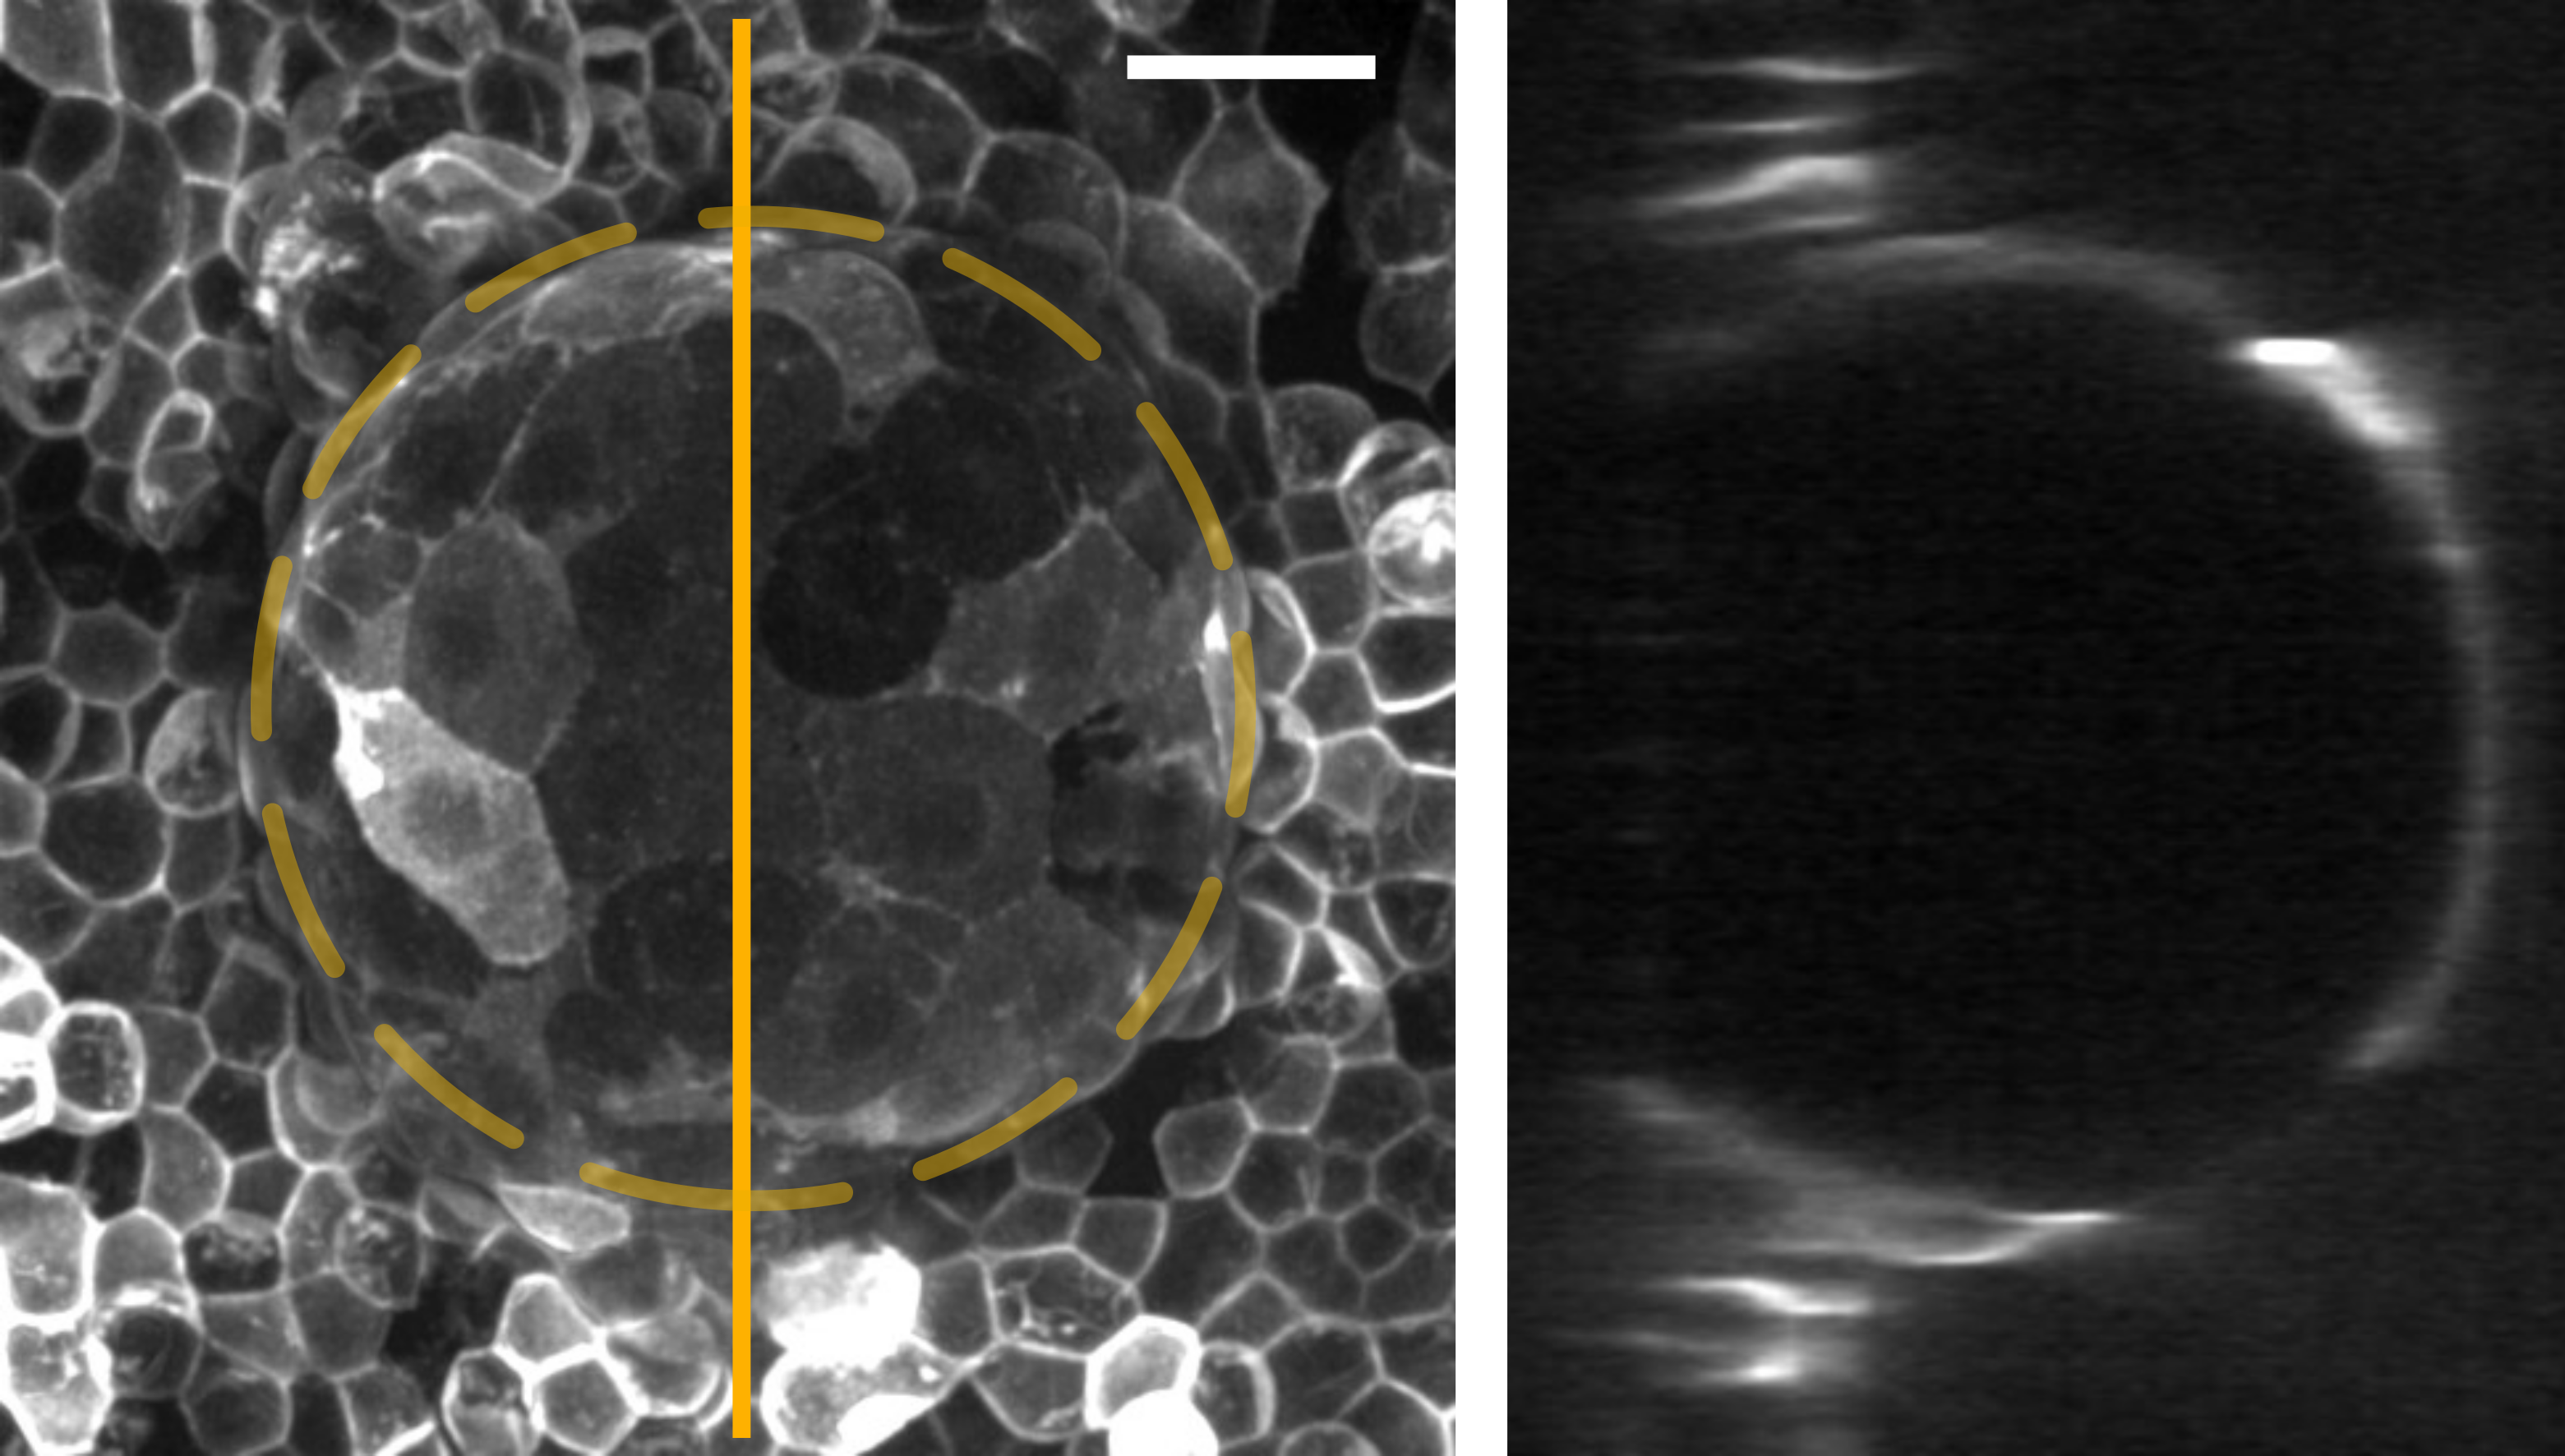
\includegraphics[width=0.8\textwidth]{chap7_realdome.png}
	\caption{\textbf{Epithelial dome generated by the MOLI device:} Maximum intensity projection of an MDCK dome (Left) . Dashed yellow line indicates the dome's footprint. Vertical yellow line crosses the center of the footprint, where the cross-section   (Right) shows the spherical shape of the dome. MDCK Cells were expressing CIBN CAAX GFP-488. Pressure, 200 Pa. Scale bar is $20 \mu m$.
	} \label{fig_7_1}
\end{figure}

\hypertarget{epithelial-domes-at-constant-pressure}{%
	\section{Epithelial domes at constant
		pressure}\label{epithelial-domes-at-constant-pressure}}

First, we systematically applied varying pressures ranging from 0-400 \unit{\pascal} to the domes. However, we observed that domes could not form at pressures lower than 50-100 \unit{\pascal} due to cell-substrate adhesion forces. Conversely, high pressures resulted in tissue delamination beyond the boundary of the patterned footprint. We determined that 200 \unit{\pascal} allowed the domes to form without delamination, falling within the previously reported pressure range \cite{choudhury2022,marin-llaurado2022}.

When domes were subjected to a constant pressure of 200 \unit{\pascal}, they underwent a significant increase in areal strain during the first three to five minutes of pressure application. Following this initial increase, the areal strain reached a plateau and remained relatively constant for the next 5-10 minutes (see Figure \ref{fig_7_3} A). Notably, our measurements also indicated considerable variability in the maximum strain achieved by domes for the same pressure, with strains ranging from 50\% to 300\%. Nevertheless, the stabilization in strain across all the domes suggested that the epithelial tissue reached a mechanical steady state.

We then plotted the tension-strain relationship of these domes, systematically finding a non-monotonic curve similar to the Nike "swoosh" symbol (see Figure \ref{fig_7_3} B). At low strains, the tension within the domes is very high, followed by a decline to a minimum value at an areal strain of 100\%, where the dome adopts a hemispherical shape. Tension then increases  again, but the rate of increase is slower than the rate at which tension decreases at lower strains. This non-monotonic tension-strain curve is at odds with previous measurements of tension-strain relations in spontaneously fluctuating domes \cite{latorre2018,marin-llaurado2022} or in cell monolayers subjected to uniaxial stretch \cite{duque2023}. The fact that strains and tensions strongly varied from dome to dome but the minimum of tension was achieved precisely at 100\% areal strain for all domes suggested that this behavior is related to the nature of our measurement. 

\begin{figure}[b!]
	\centering
	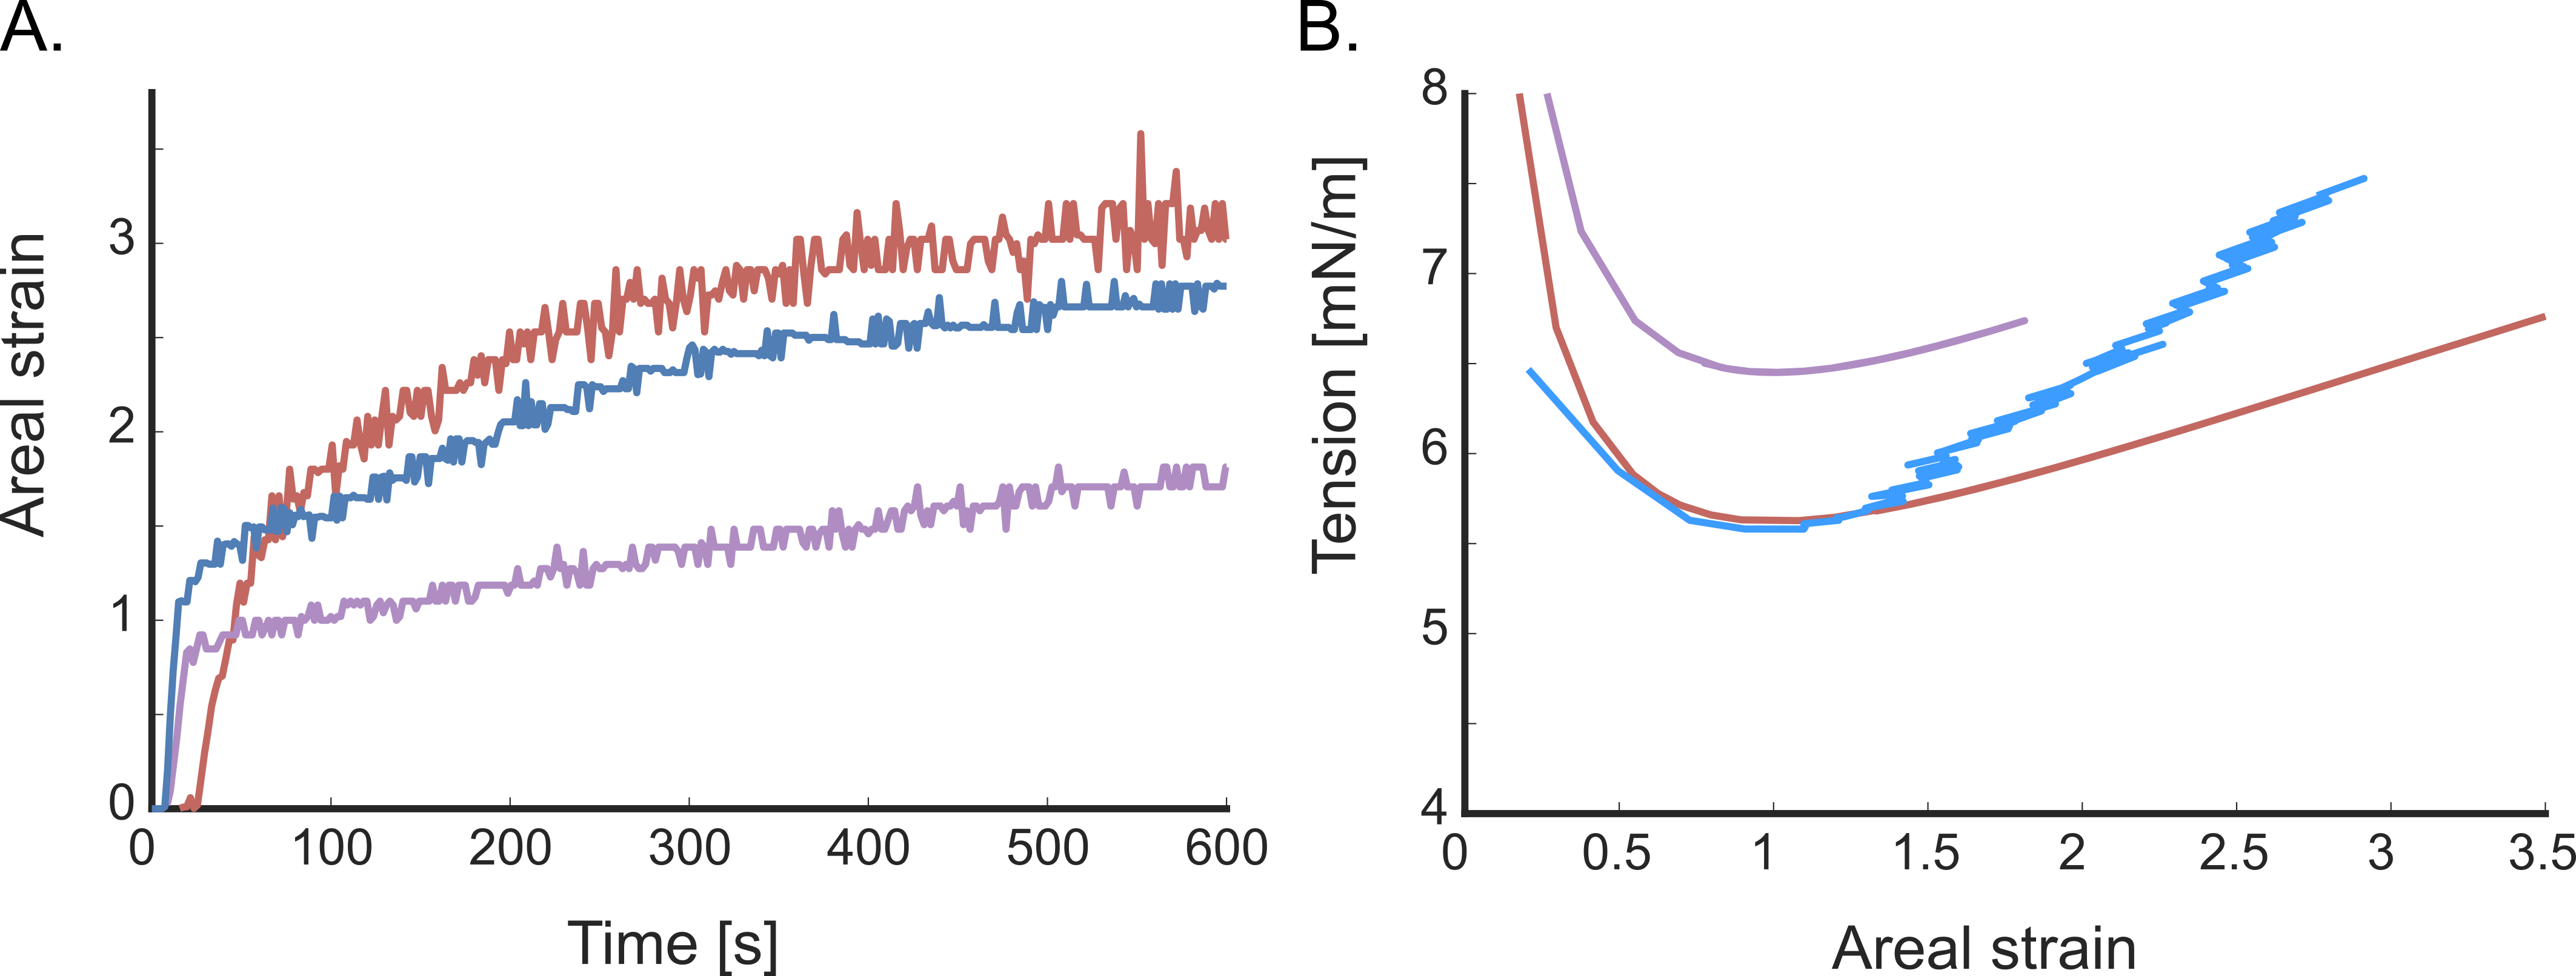
\includegraphics[width=\textwidth]{chap7_constpressure.png}
	\caption{\label{fig_7_3} \textbf{Epithelial domes at constant pressure}: Dynamic response of three representative domes at a constant pressure of 200 Pa \marino{[specify the basal radius for each dome]}: (A) Areal strain increases and reaches a steady state at around 5 minutes, and we can clearly see variability in the maximum strains. (B) The same domes produce a peculiar tension and strain curve. (representative of 12 domes)
	}
\end{figure}

Our measurement of the stress-strain relation only uses (1) mechanical equilibrium, encoded by Laplace's law, and (2) the geometrical relations between the radius of curvature $R$ of the dome, the footprint radius $a$, the height $h$ and the areal strain $\epsilon$. The geometric Eqs.~(\ref{eqn:radiuscurve},{eqn:arealstrain}) can be combined to find an explicit relation between radius of curvature and strain
\begin{equation}
	R = \frac{h^2/a^2 + 1}{2h/a^2} = a\frac{\epsilon + 1}{\sqrt{\epsilon}},
\end{equation}
which when plugged into Laplace's law in Eq.~(\ref{eqn:laplace}) results in 
\begin{equation}
	\label{eqn:isobaric}
	\frac{\sigma}{a \Delta P} = \frac{1}{4}  \frac{\epsilon + 1}{\sqrt{\epsilon}}.
\end{equation}
This relation relates two non-dimensional quantities. Since in the experiments reported in Figure \ref{fig_7_3} pressure $\Delta P$ and footprint radius $a$ are constant, this relation shows that tension should be proportional to $(\epsilon + 1)/\sqrt{\epsilon}$ irrespective of the mechanical response of the tissue, as a result of geometry and mechanical equilibrium. For small strains ($\epsilon\ll 1$), we have $\sigma \propto 1/\sqrt{\epsilon}$, whereas for large strains $\epsilon\gg 1$, we have $\sigma \propto \sqrt{\epsilon}$ in agreement with the non-monotonic measured stress-strain curves. A geometric interpretation of the isobaric curve is shown in Figure \ref{fig_7_4}, which reflects the fact that the radius of curvature of a spherical dome of fixed footprint is minimum when the dome is half sphere. When represented according to Eq.~(\ref{eqn:isobaric}), all tension-strain curves collapse to a master curve reflecting the hypotheses of the measurement \marino{[Show as inset??]}.



%The tension-strain relationship of the domes can be explained by the geometric constraints imposed by the dome system and force balance. Laplace’s law implies that for a constant pressure, the tension within the dome is directly proportional to its radius of curvature. Domes with low strain are close to being flat monolayers and have a high value of the radius of curvature, which leads to a correspondingly high tension  (see Figure \ref{fig_7_4}). As the dome inflates, the radius of curvature subsequently diminishes to a minimum upon adopting a hemispherical shape. Since the dome always maintains a spherical shape, the radius of curvature, areal strain, and tension are all interconnected. The curve's expression can be derived by substituting areal strain ($\epsilon$) in the expression of radius of curvature ($R$) (Equation \ref{eqn:radiuscurve})


The previous discussion shows that Eq.~(\ref{eqn:isobaric}) alone does not say anything about the mechanical response of the epithelial monolayer. However, the fact that domes plateau to a steady-state strain, and hence to a plateau tension according to the isobaric relation Eq.~(\ref{eqn:isobaric}), provides a measurement of a $(\epsilon, \sigma)$ pair at steady state. In the next section, we discuss how to use this principle to measure 


These measurements imply that when a step pressure is applied, the inflating dome undergoes a non-steady-state with out-of-equilibrium stresses while experiencing high tension related to high radius of curvature. The dome then rapidly inflates by following the tension-strain curve dictated by equation \ref{eqn:isobaric} to achieve a steady state. In this steady state, the external pressure is balanced with equilibrium tissue tension. It is evident that this tension-strain curve observed does not represent the quasi-static material response of the epithelial tissue. To determine the true tension strain relation, a different experimental strategy will be adopted in the following section.

\begin{figure}
	\centering
	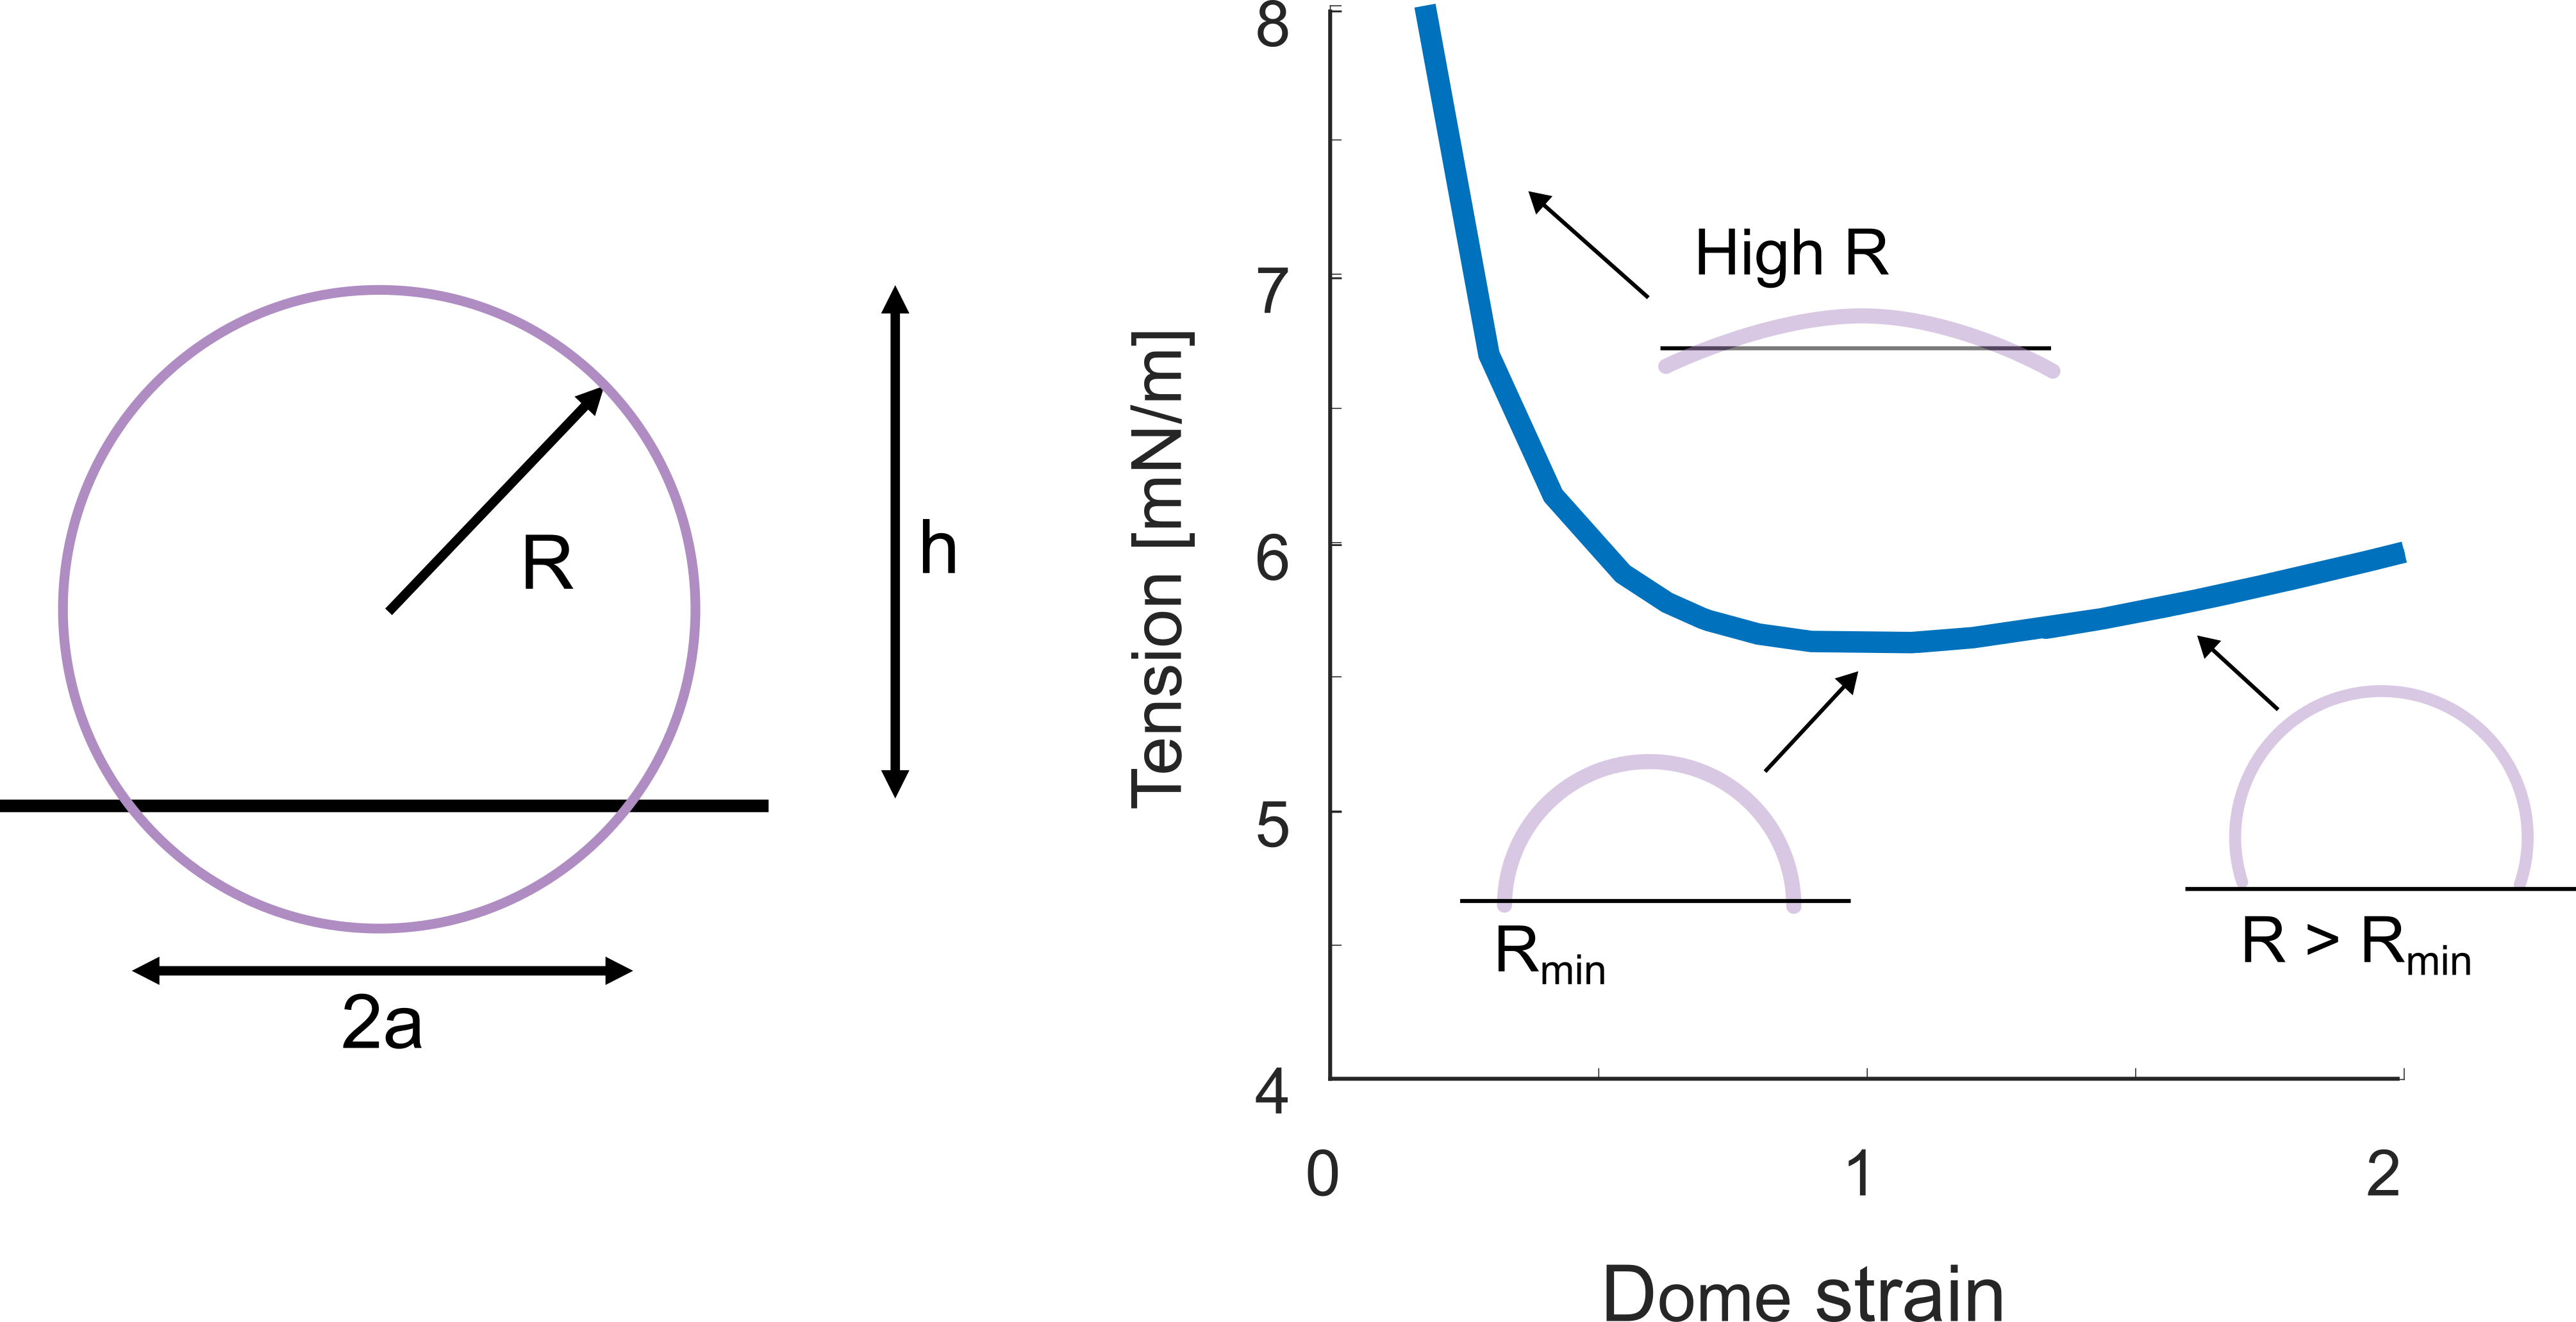
\includegraphics[width=0.8\textwidth]{chap7_radius.png}
	\caption{\label{fig_7_4} \textbf{Illustrative explanation for isobaric curve}: Tension and strain are related to each other through the geometric constraint of a spherical cap. Here, the base radius (a) is constant, so the radius of curvature is almost infinite for domes with very small strains (<0.05). As the strain increases, the radius of curvature decreases to a minimum corresponding to the base radius. Then it continues to increase again.	
	}
\end{figure}

\hypertarget{constitutive-relation-of-epithelia}{%
	\section{Constitutive relation of
		epithelia}\label{constitutive-relation-of-epithelia}}

The constitutive relation of a material describes the relationship between its deformation and the applied forces. In conventional material testing, quasi-static strain or tension is applied to determine this relation. However, our experiments could only control pressure. Increasing pressure quasi-statically was not feasible for domes due to limited delamination at low pressures. To overcome this and obtain the tissue constitutive relation, we deflated a dome in steps, capturing steady-state tension and strain for different pressures.

Specifically, we applied a pressure of 200 \unit{\pascal} for 5 minutes, allowing the dome to reach a steady state. We then reduced the pressure in increments of 20 \unit{\pascal}, permitting the dome to reach steady state at each step (see Fig. \ref{fig_7_5}). This process continued until the dome was completely deflated. Through this approach, we captured the material response of the tissue at various pressures as the dome transitioned through different tension-strain states. By mapping all steady-state tension-strains of domes at different pressures, we determined a constitutive relation for the tissue.

The resulting constitutive relation showed an initial increase in tension with strain for lower strains. For larger strains, the tension plateaued, consistent with earlier studies on MDCK domes (see Fig. \ref{fig_7_5} B). It is important to note the significant variability in dome-to-dome tension, with recorded tensions around 4.5 \unit{mN/m} consistent with the same order of magnitude as those in previous studies \cite{latorre2018,marin-llaurado2022}.

\begin{figure}[b!]
	\centering
	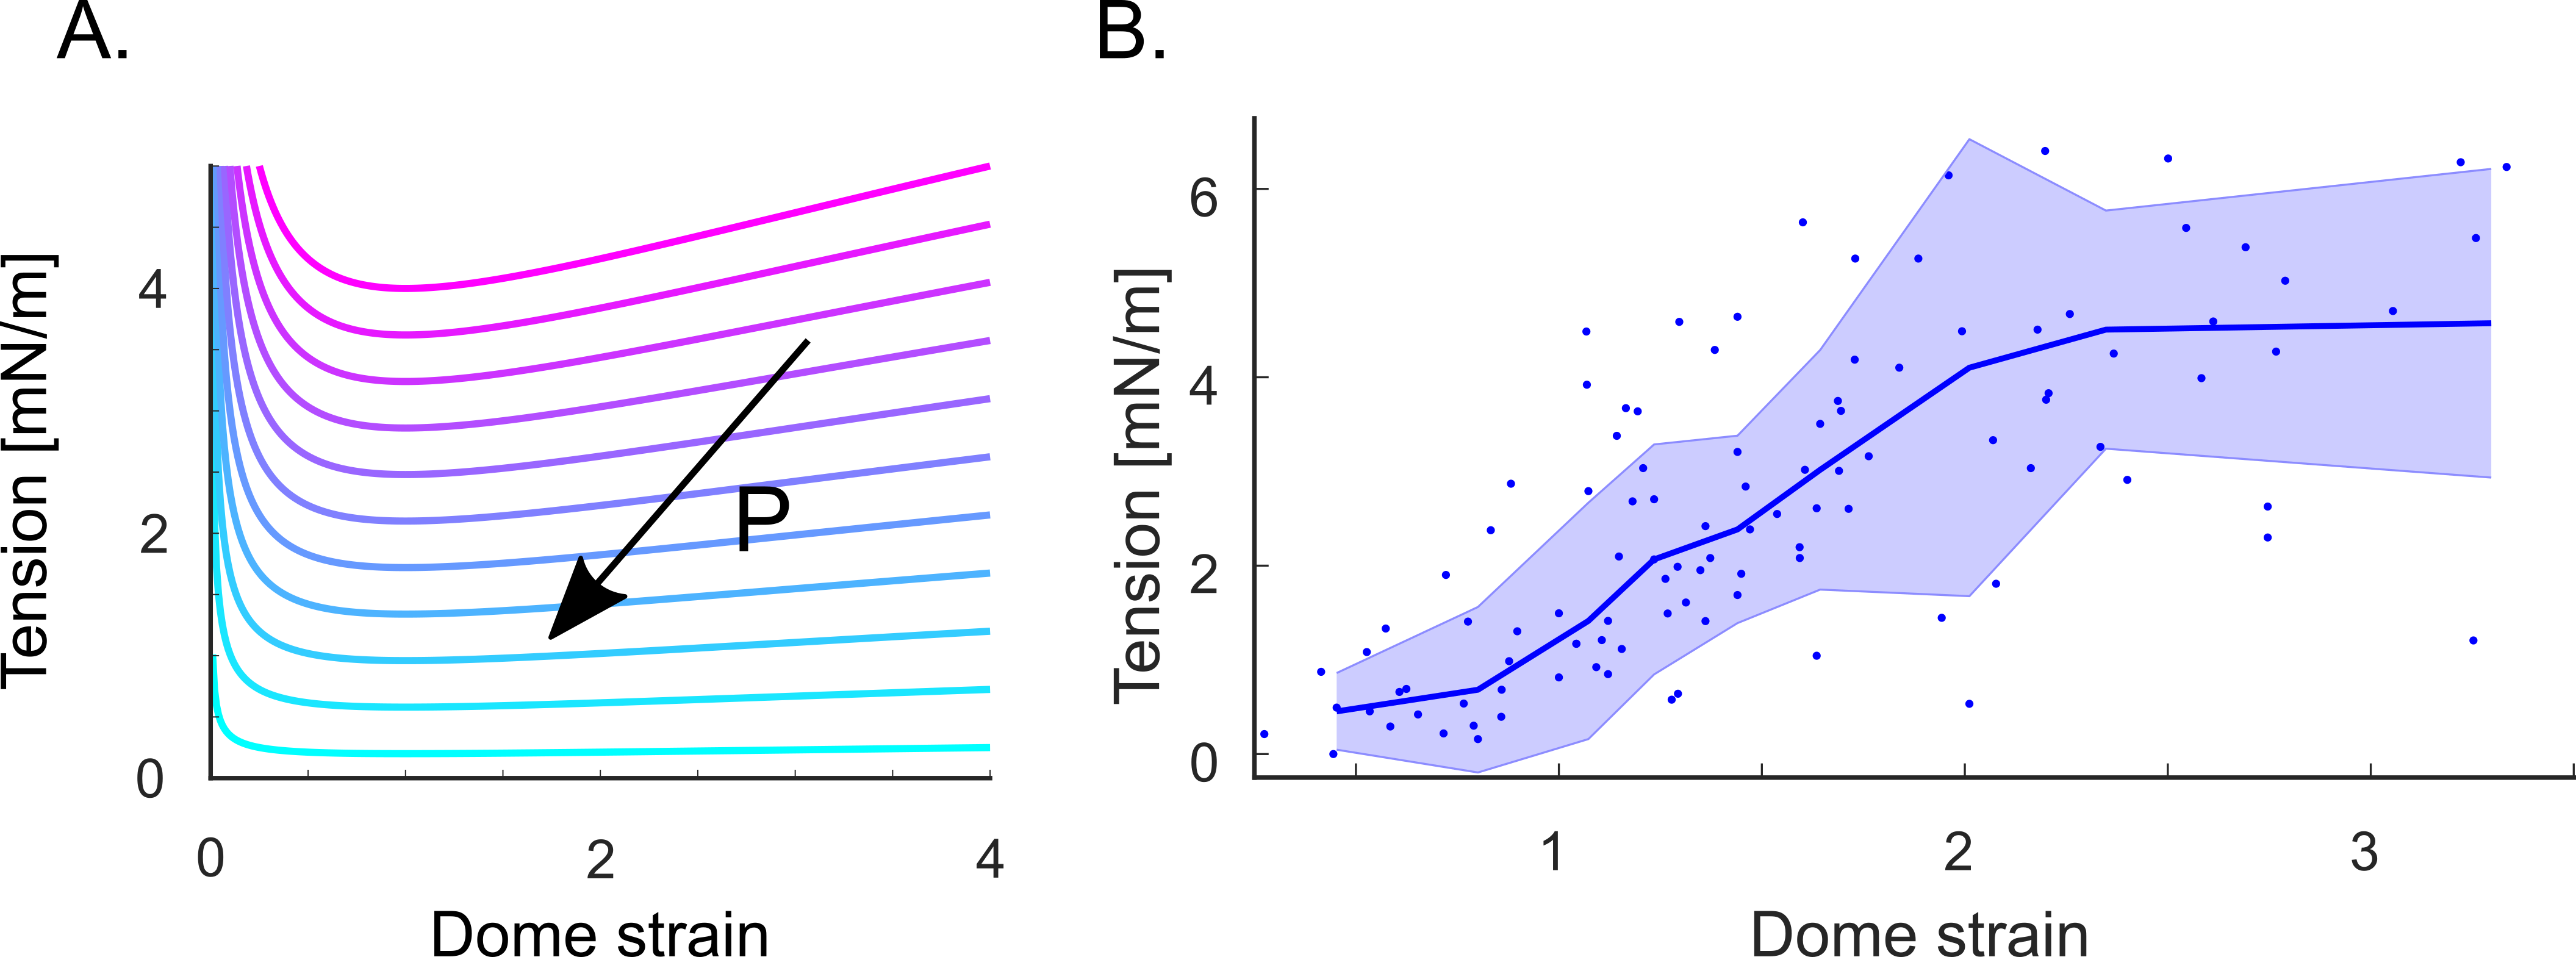
\includegraphics[width=\textwidth]{chap7_constitutivelaw.png}
	\caption{\label{fig_7_5} \textbf{Constitutive Relation of Epithelia}: (A) We set up experiments to probe the steady state at different pressures. We will start from the highest pressure, move along the isobaric line and achieve a steady state, and then move down to the next curve, and so on.	(B) The constitutive relation between dome strain and tissue tension was experimentally obtained (n=12). The line and shaded area represent the median and standard deviation, respectively, by binning 13 points in each bin.}
\end{figure}

To summarize, our experiments demonstrate that the tissue reaches a steady state under a specific static pressure, which enables us to determine its constitutive relation through deflation. In the next section, we will explore the dynamic material response of the tissue.

\vspace{0cm}

\hypertarget{dynamics-of-the-epithelia-domes}{\section{Dynamics of the epithelial domes}\label{dynamics-of-the-epithelial-domes}}

In this section, we investigated the dynamic material response of the domes by conducting cyclic stretching experiments. We subjected the domes to a triangular wave of pressure with a magnitude of 200 Pa at three distinct timescales, as depicted in Figure \ref{fig_7_6} A. The selected timescales of 20s, 266s, and 2000s were based on existing literature on tissue remodeling, particularly the work of Khalilgharibi et al. (2019) and Casares et al. (2015) \cite{khalilgharibi2019, casares2015}. These studies demonstrated that stress relaxation in tissues occurs from tens of seconds to minute timescales due to F-actin remodeling and myosin-driven contractility. Additionally, in some cases, even faster deformation at timescales of a few seconds has been shown to impact cell remodeling \cite{andreu2021a}. In our device, the fastest cycle that could be probed was limited to 20s because of the microscope’s imaging speed.

\begin{center}
	\begin{table}[h!]
		\label{tab:hysteresis}
		\centering
		\begin{tabular}{c c c c}
			& Fast & Moderate & Slow \\ 
			Time period (s) & 20   & 266      & 2000 \\ 
			Rates (Pa/s)    & 20   & 1.5      & 0.2  \\ 
		\end{tabular}
		\caption{Pressure rates used for cyclic stretching experiments}
	\end{table}
\end{center}

For the fastest cycles, we observed that the maximum strain achieved by the domes in each cycle increased until they reached a steady state oscillation around 600 seconds. The experiment was conducted over 1200 seconds, equivalent to 60 cycles, during which we observed a cumulative buildup of strain over time. In the loading phase, the domes underwent stretching, while during the unloading phase, they experienced unstretching but failed to revert to zero strain after the initial cycles. In the concluding cycles, we noted that the dome oscillated between two distinct states of strain, resembling a limit cycle (see Figure \ref{fig_7_6} B top).

A similar response was observed for the moderate cycles, where the domes were stretched for five cycles of 266s each. The strain accumulated in the first cycle, with strains reaching higher values than those observed in the fast case (see Figure \ref{fig_7_6} B middle). Moreover, after a few cycles, the dome appeared to reach a stable limit cycle.

In the slowest loading experiments, two cycles of 2000s, we observed that the domes did not form at lower pressures. As discussed earlier, the domes remained attached until a pressure of 100-150 Pa was attained, beyond which they underwent rapid inflation, leading to high strains of 200-350\%. However, during cyclic stretching, we noted that strain accumulation did not occur, and there was no variation in the maximum strains attained during both cycles (see Figure \ref{fig_7_6} B bottom). The cells were able to stretch four times their original size and return to the original size at the end of each cycle.

These experiments clearly demonstrated the rate-dependent response of the domes, with faster rates resulting in strain accumulation and slower rates allowing for reversible large deformations. This behavior is indicative of viscoelasticity. In the next section, we will explore this viscoelastic behavior with help of a computational model.

\begin{figure}[]
	\centering
	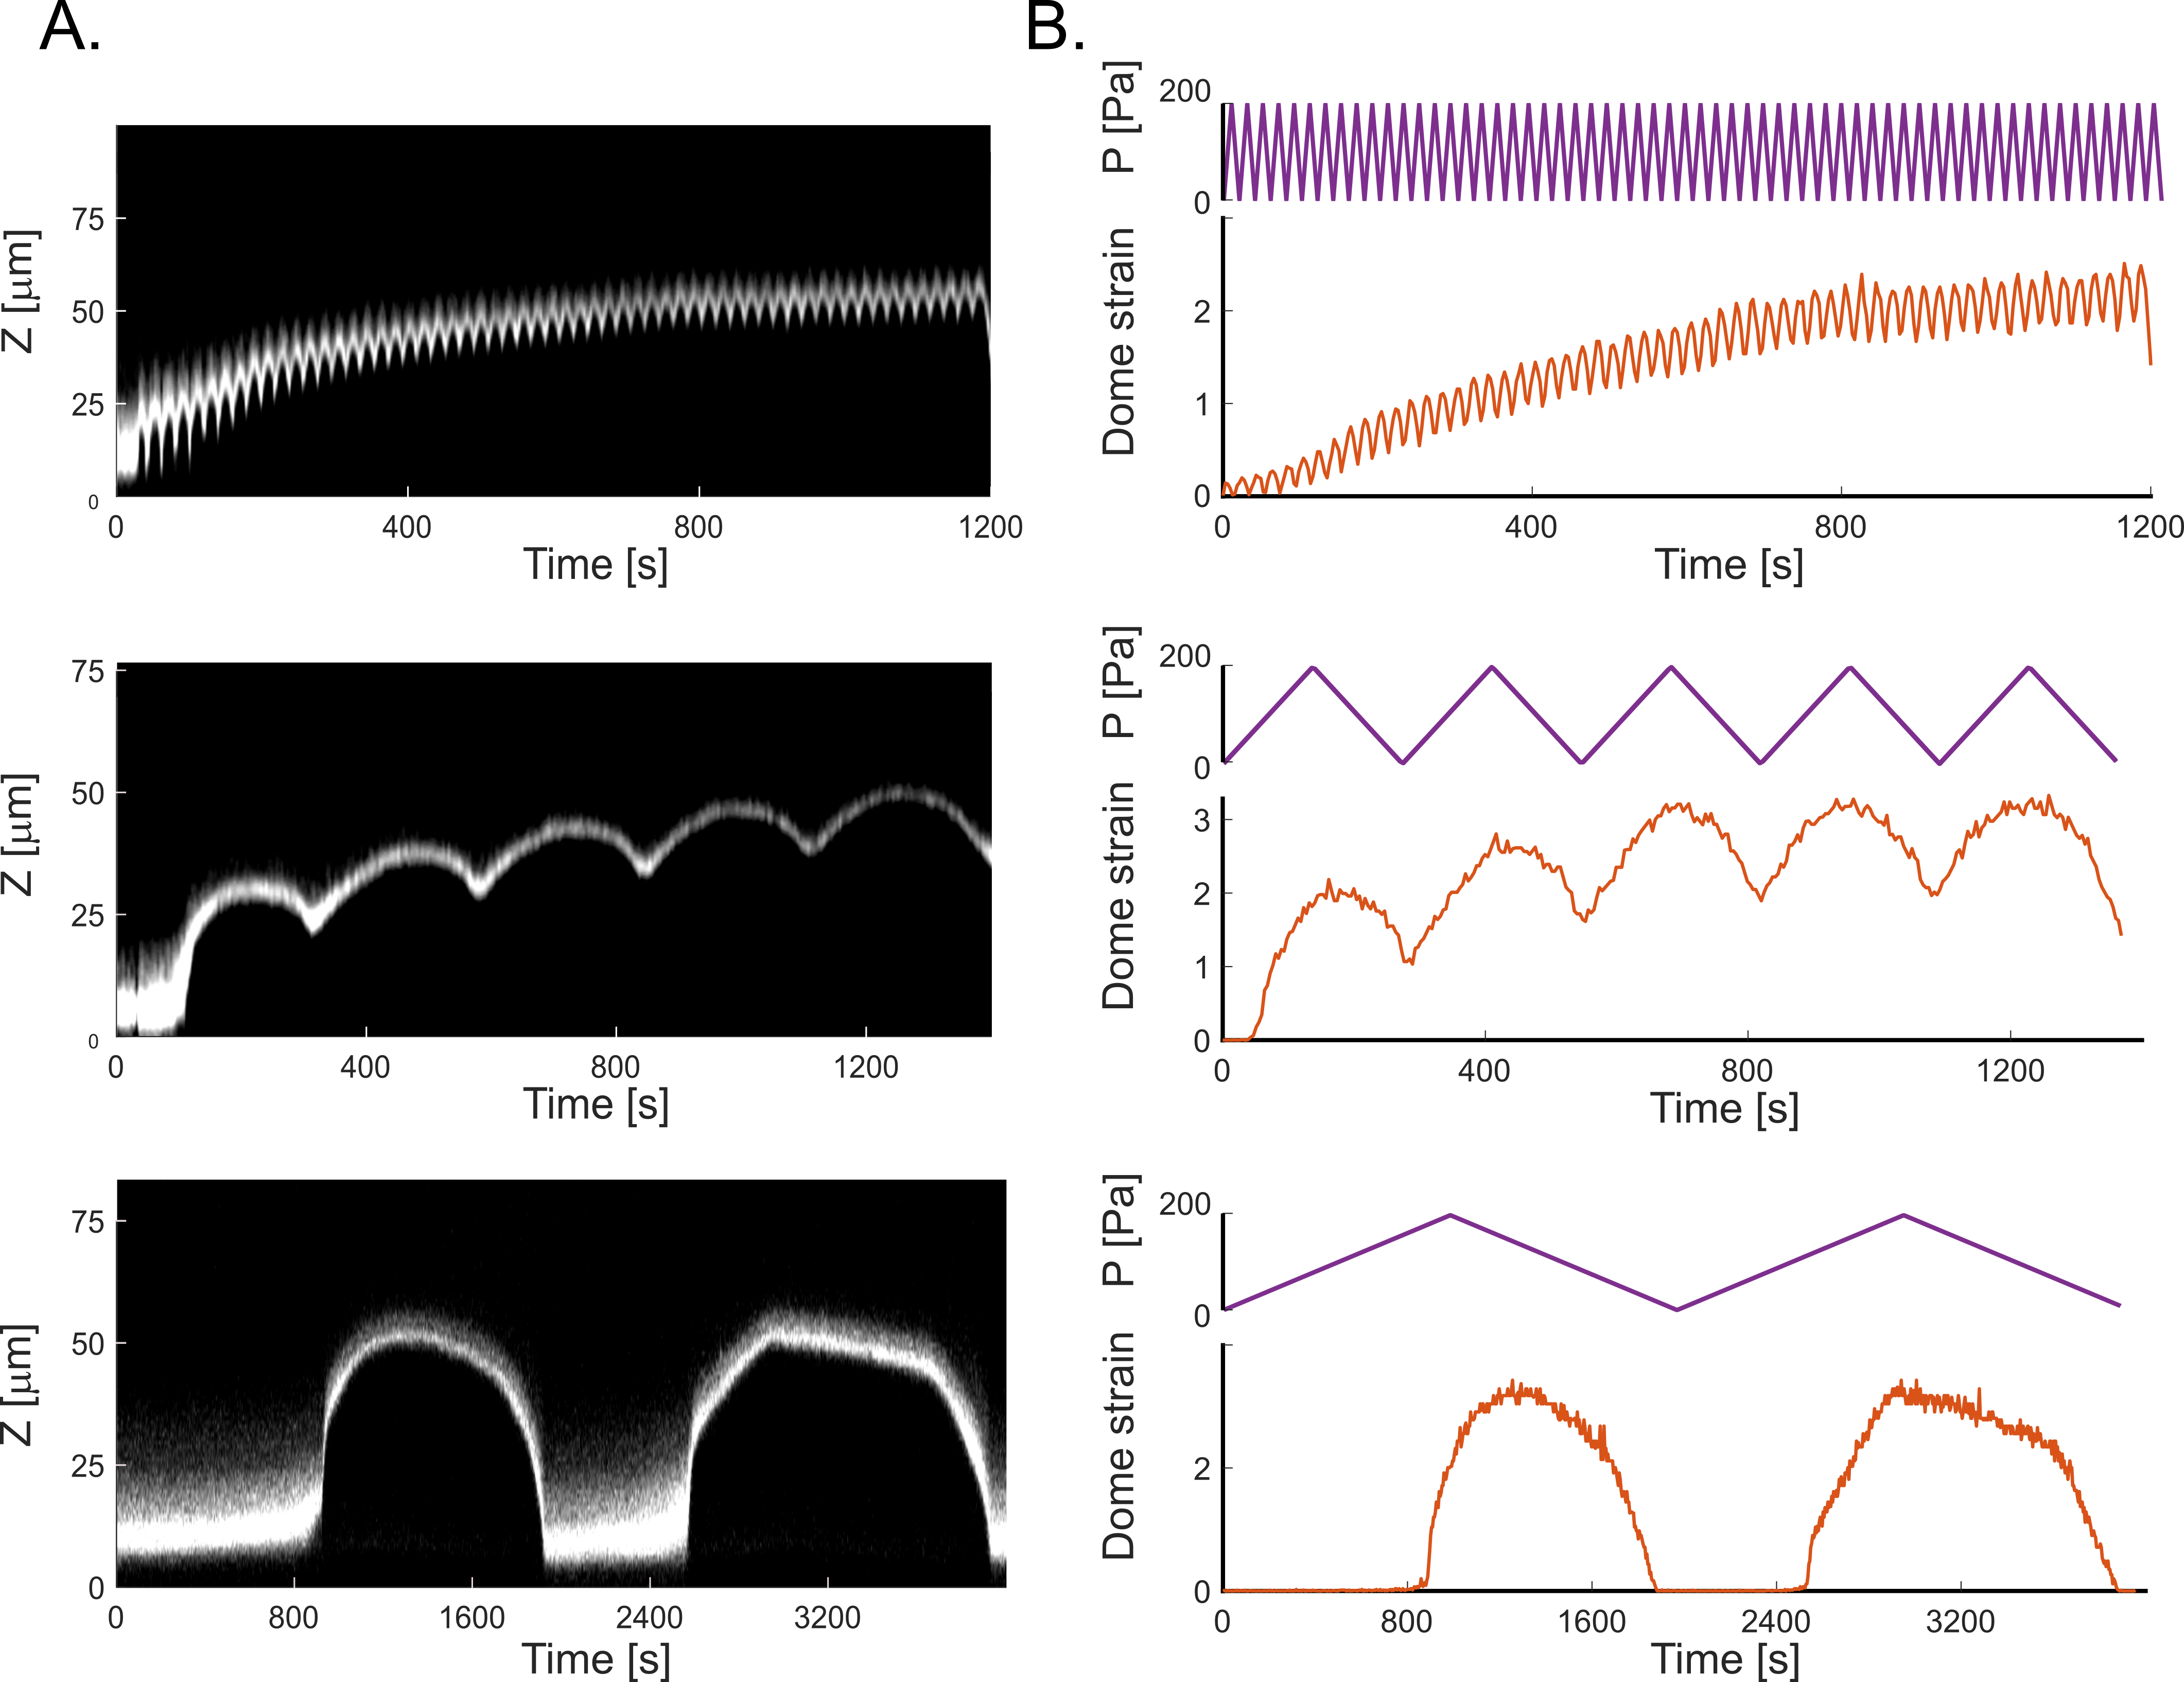
\includegraphics[width=\textwidth]{chap7_dynamic.png}
	\caption{\label{fig_7_6} \textbf{Dynamic response of Epithelia:} (A) The XZ plane images and kymographs of domes subjected to cyclic pressure between 0 to 200 Pa with rates of 20, 1.5, and 0.2 Pa/s The kymographs generated along the midsection of the domes indicated by yellow dotted lines. These indicate the evolution of height of the domes with respect to time. (B) The strain response of domes to cyclic pressure with different rates. Magenta represents pressure and red represents strain with respect to time. For A, B, n= 7 domes for 20 Pa/s, n = 8 for 1.5 Pa/s, and n = 7 for 0.2 Pa/s. 
	}
\end{figure}

\newpage

\hypertarget{active-gel-tissue-model}{%
	\section{Active gel tissue model}\label{active-gel-tissue-model}}

Current literature emphasizes that the response of the cell to deformations over various time scales is governed by the viscoelasticity of the actin cortex \cite{kelkar2020, clement2017, khalilgharibi2019}. To further understand this behavior, Adam Ouzeri and Marino Arroyo developed a computational model that bridges active gel models of the actomyosin cortex with 3D vertex models at tissue scales \cite{ouzeri2023}. Our collaboration necessitated close coordination, with Adam Ouzeri developing the model and me conducting experiments, facilitating the effective integration of the model with experimental data.

The model simplifies the complex cortex, comprising the actin filament network, hundreds of actin-binding proteins, and myosin motors, into a thin layer of contractile gel. This layer possesses a thickness denoted as cortical thickness (\(\rho\)).

The crosslinked actin filament network exhibits the behavior of an elastic network of semi-flexible filaments, whose material properties are represented by Lamé parameters  (\(\lambda,\mu\)). Consequently, upon deformation, it can store elastic energy, at shorter timescales. At longer timescales, in response to stretching, the network dynamically reorganizes itself, releasing the stored elastic energy by relaxing stresses. This takes place through assembly/disassembly of the filaments or binding/unbinding of the crosslinkers. The dissipation of stresses is represented by a viscosity coefficient (\(\eta\)).

The active component of the active gel model arises from myosin motor activity, generating contractile active tension in the network. This active tension (\(\gamma\)) is hypothesized to be directly proportional to cortical thickness:	$\gamma(\rho) = \xi \rho$, with a proportionality constant denoted by coefficient of active tension (\(\xi\)).

Several assumptions underlie this model. Firstly, it is assumed that the cell volume remains conserved throughout the deformations. Secondly, it is understood that cells cannot stretch indefinitely. To limit strains, a strain stiffening mechanism is introduced, which is activated at high strains. With respect to the actin network, it is assumed to be isotropic and undergoes constant turnover, thereby maintaining a steady-state cortical thickness.

Based on the above assumptions and the cortex’s physical attributes, the model represents each cell as an active gel surface. These active gel surfaces are then assembled to form a tissue, as depicted in Figure \ref{fig_7_2}. The system’s dynamics are formulated through a balance of diverse potentials, representing free energy, dissipation, active contractility, and external forces.

Due to this formulation, three timescales emerge from the theoretical framework: 

\begin{enumerate}
	\item Turnover timescale \(t_{to} = 1/k_{d}\)
	\item Viscoelastic timescale \(t_{ve} = \eta/\lambda\)
	\item Viscoactive timescale \(t_{va} = \eta/\xi\)
\end{enumerate}

The turnover timescale is driven by the cortex's polymerization rates (\(k_{d}\)). The viscoelastic timescale is a ratio of the viscous remodeling coefficient to the Lamé parameters, representing elasticity. Lastly, the viscoactive timescale is the ratio of the viscous remodeling coefficient to the coefficient of active tension. All of these timescales are interconnected through the cortical thickness; thus, for simplicity, we can understand them as one remodeling timescale

Using this model, a virtual representation of a cell monolayer can be generated, with specific boundary conditions. In particular, we can create a cell monolayer with regions that lack basal attachment to the substrate, which can be inflated into domes under pressure application, similar to the experimental setup. These simulations will be referred to as "digital domes" in subsequent discussions  (see Figure \ref{fig_7_2}). By employing this model and comparing the results with the experimental data, we can effectively understand and investigate the biomechanical properties of epithelial tissues, specifically the contribution of the viscoelasticity of the actin cortex.

\begin{figure}[]
	\centering
	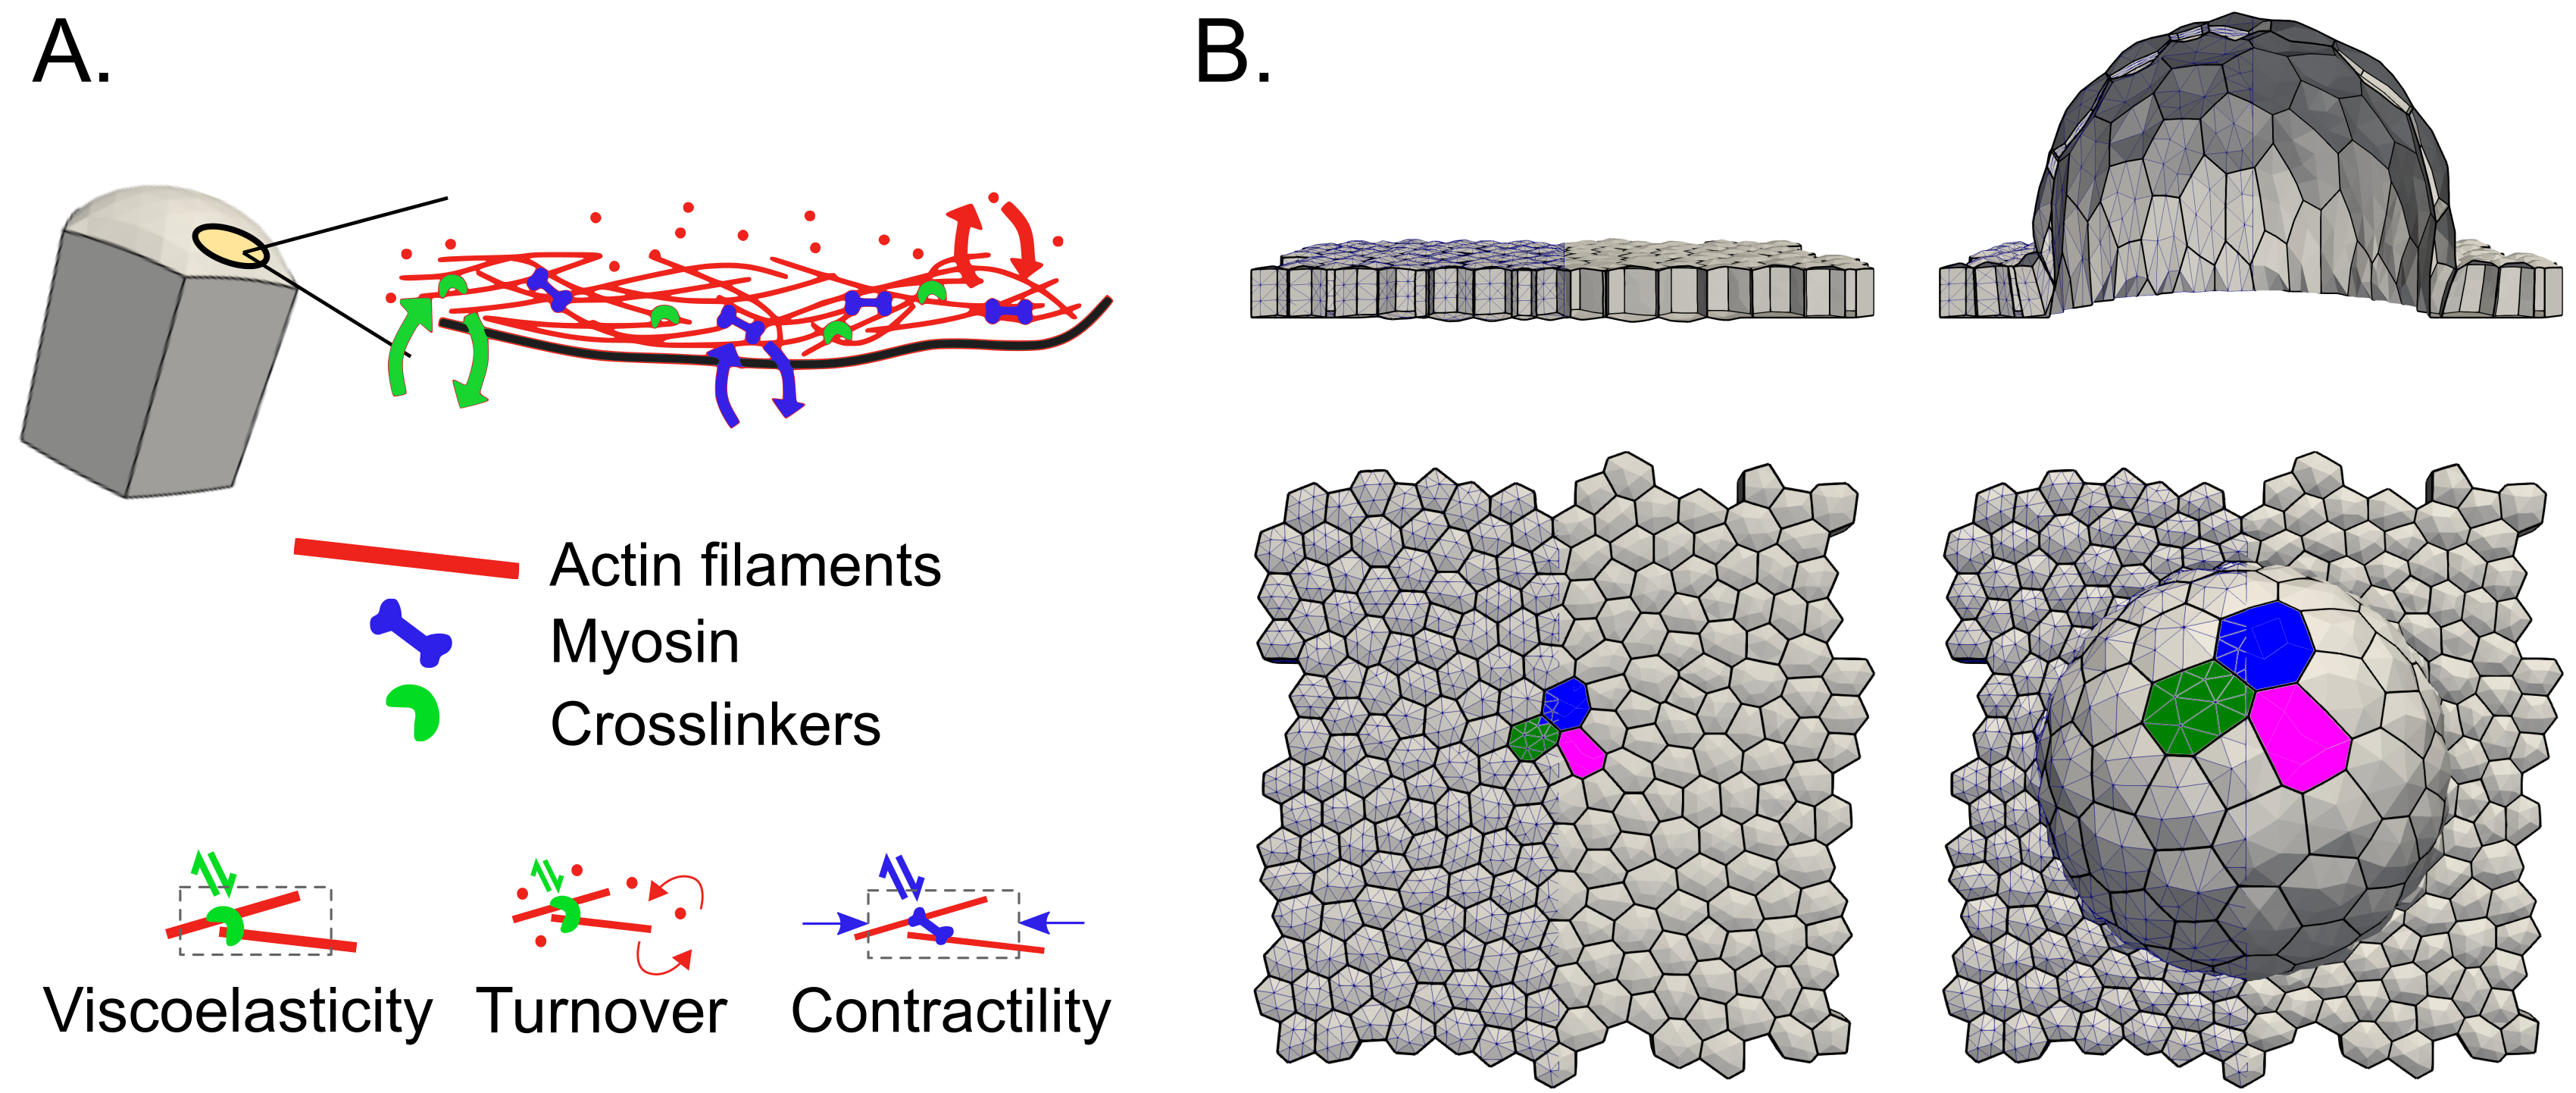
\includegraphics[width=\textwidth]{chap7_digitaldome.png}
	\caption{\label{fig_7_2} \textbf{Active gel tissue model}: (A) The cell is modeled as an active gel of cortex, which mainly comprises three aspects: viscoelasticity of the network, turnover dynamics, and active contractility. (B) These cells can be assembled into a tissue that can be used to perform in-silico experiments. An example of this is the digital dome being inflated, color is highlighting individual cells increasing their area.}
\end{figure}

\hypertarget{active-viscoelasticity-of-the-epithelia}{%
	\section{Active viscoelasticity of the
		epithelia}\label{active-viscoelasticity-of-the-epithelia}}
	
In this section, we interpret the experimental results within the context of the active gel tissue model. The mathematical framework describes how cells, represented as an active gel, change shape. Specifically, the initial shape, known as the reference configuration (\(\Gamma_{0}\)), is mapped to its current shape, called the deformed configuration (\(\Gamma\)). This mapping enables the quantification of strains and deformations relative to the reference configuration using a metric tensor, which measures distances and angles within the material. When a material is deformed, the distances and angles within it change, and the metric tensor reflects these changes. In this case, each configuration possesses its own metric tensor.

For typical elastic materials, the reference configuration remains fixed in time, and deformations are measured relative to this fixed state. However, to account for the remodeling of the cortex through dynamic crosslinking, our model considers the reference configuration as dynamic, necessitating a time-varying metric tensor  (\(\mathbf{G}\)). We can refer to this evolving reference configuration as the resting frame. By employing the dynamic metric tensor, we can calculate the resting area of a cell, which represents an imagined area where all stored elastic energy is dissipated. In terms of cell area, the relationship between the resting area (\(A_{rest}\)) and the actual area (\(A_{actual}\)) can be expressed as

\begin{equation}
	A_{rest} = \int_{\Gamma_0} \sqrt{|\mathbf{G}|}dS_0, \text{ and } A_{actual} = \int_{\Gamma}dS.
\end{equation}

Where $dS_{0}$ and $dS$ are infinitesimal area on the cortex in
reference and deformed configuration respectively.

In the case of a polymer with dynamic crosslinks, the resting area of the material changes as the crosslinks break and reform in response to applied stress. The updated resting area can be used as a dynamic reference configuration for measuring subsequent deformations of the material.

Consider an example where the tissue is step stretched biaxially. The actual area changes instantly, but the resting area of the tissue stretches gradually and eventually becoming equal to the actual area due to the active viscoelasticity of the tissue (see Figure \ref{fig_7_7a} A). This process involves two types of stresses: viscoelastic stress and active tension. The total tissue tension is the sum of these two stresses. Upon stretching the tissue, viscoelastic stresses dissipate at viscoelastic timescales through remodeling, which allows the resting area to match the actual area, while active tension increases at turnover timescales (see Figure \ref{fig_7_7a} B). The effect of this remodeling on the tissue behavior is evident in experiments described in previous sections.

\begin{figure}[b!]
	\centering
	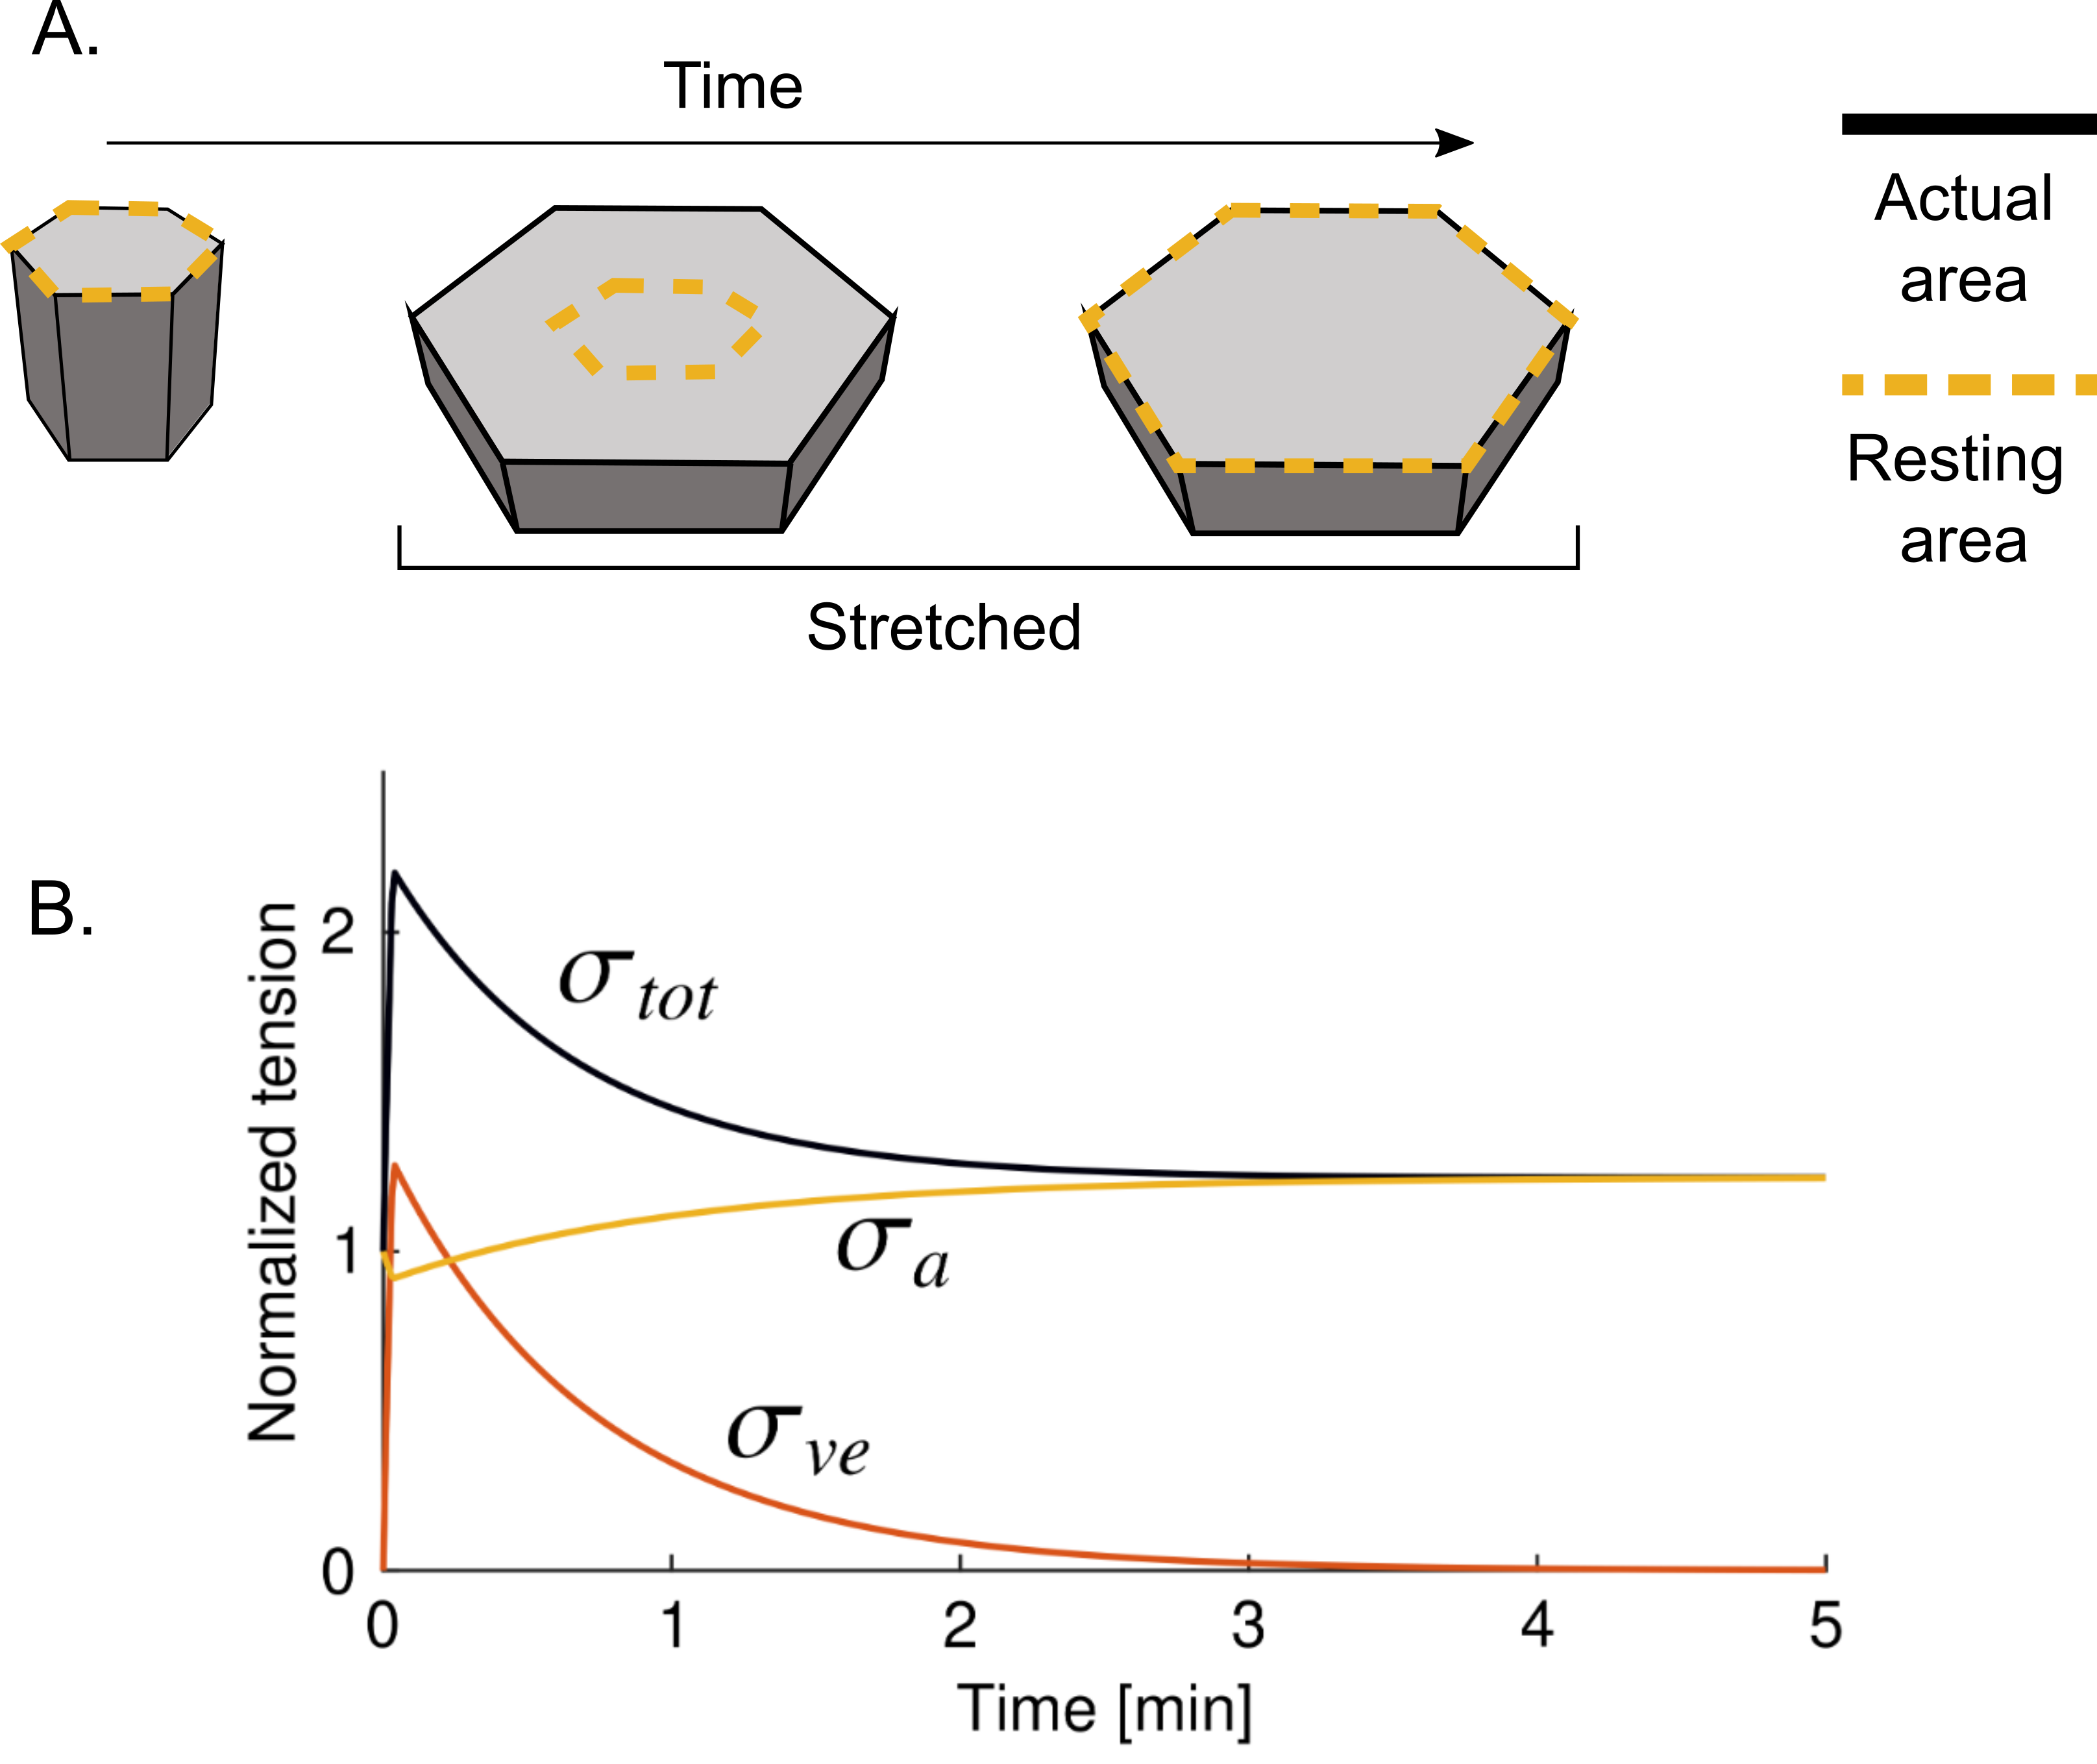
\includegraphics[width=0.8\textwidth]{chap7_area1.png}
	\caption{\label{fig_7_7a} \textbf{Viscoelastic remodeling after step deformation leads to relaxation}: (A) Illustration of a resting and actual are of a cell in a tissue during stretching. (B) Evolution of total tissue tension (black), viscoelastic stress (red), and active tension (yellow) in response to step deformation.
	}
\end{figure}

The simulations were conducted to mirror the experimental conditions. Upon subjecting the digital dome to constant pressure, consistent with our previous experimental observations, the digital dome reached a steady state while experiencing a reduction in cortical thickness as the cells stretched (refer to Figure \ref{fig_7_7}). The remodeling of the cortex dissipates the viscoelastic stress and increases the active tension. At the steady state point, only the active tension remains balancing the externally applied pressure. The simulations show that the time to reach the steady state is mainly driven by the viscoelastic timescales. The tension-strain relationship of the digital domes also produced a non-monotonous tension-strain curve observed in experiments (refer to Figure \ref{fig_7_7}).

To derive the proper constitutive relation within the computational framework, the digital dome was subjected to quasi-static inflation. The resulting constitutive curve displayed characteristics similar to those observed experimentally, and additionally, exhibited stiffening at high strains, which can be attributed to a barrier mechanism introduced to limit high strains (see Figure \ref{fig_7_7} A).

Furthermore, to assess the robustness of the constitutive relation obtained from our experiments, the digital dome was inflated to varying levels of pressure, generating tension-strain curves and steady-state points. The locus of steady-state points under different constant pressure conditions aligned with the quasi-statically obtained constitutive relation, as illustrated in Figure  \ref{fig_7_7} B.


\begin{figure}[t]
	\centering
	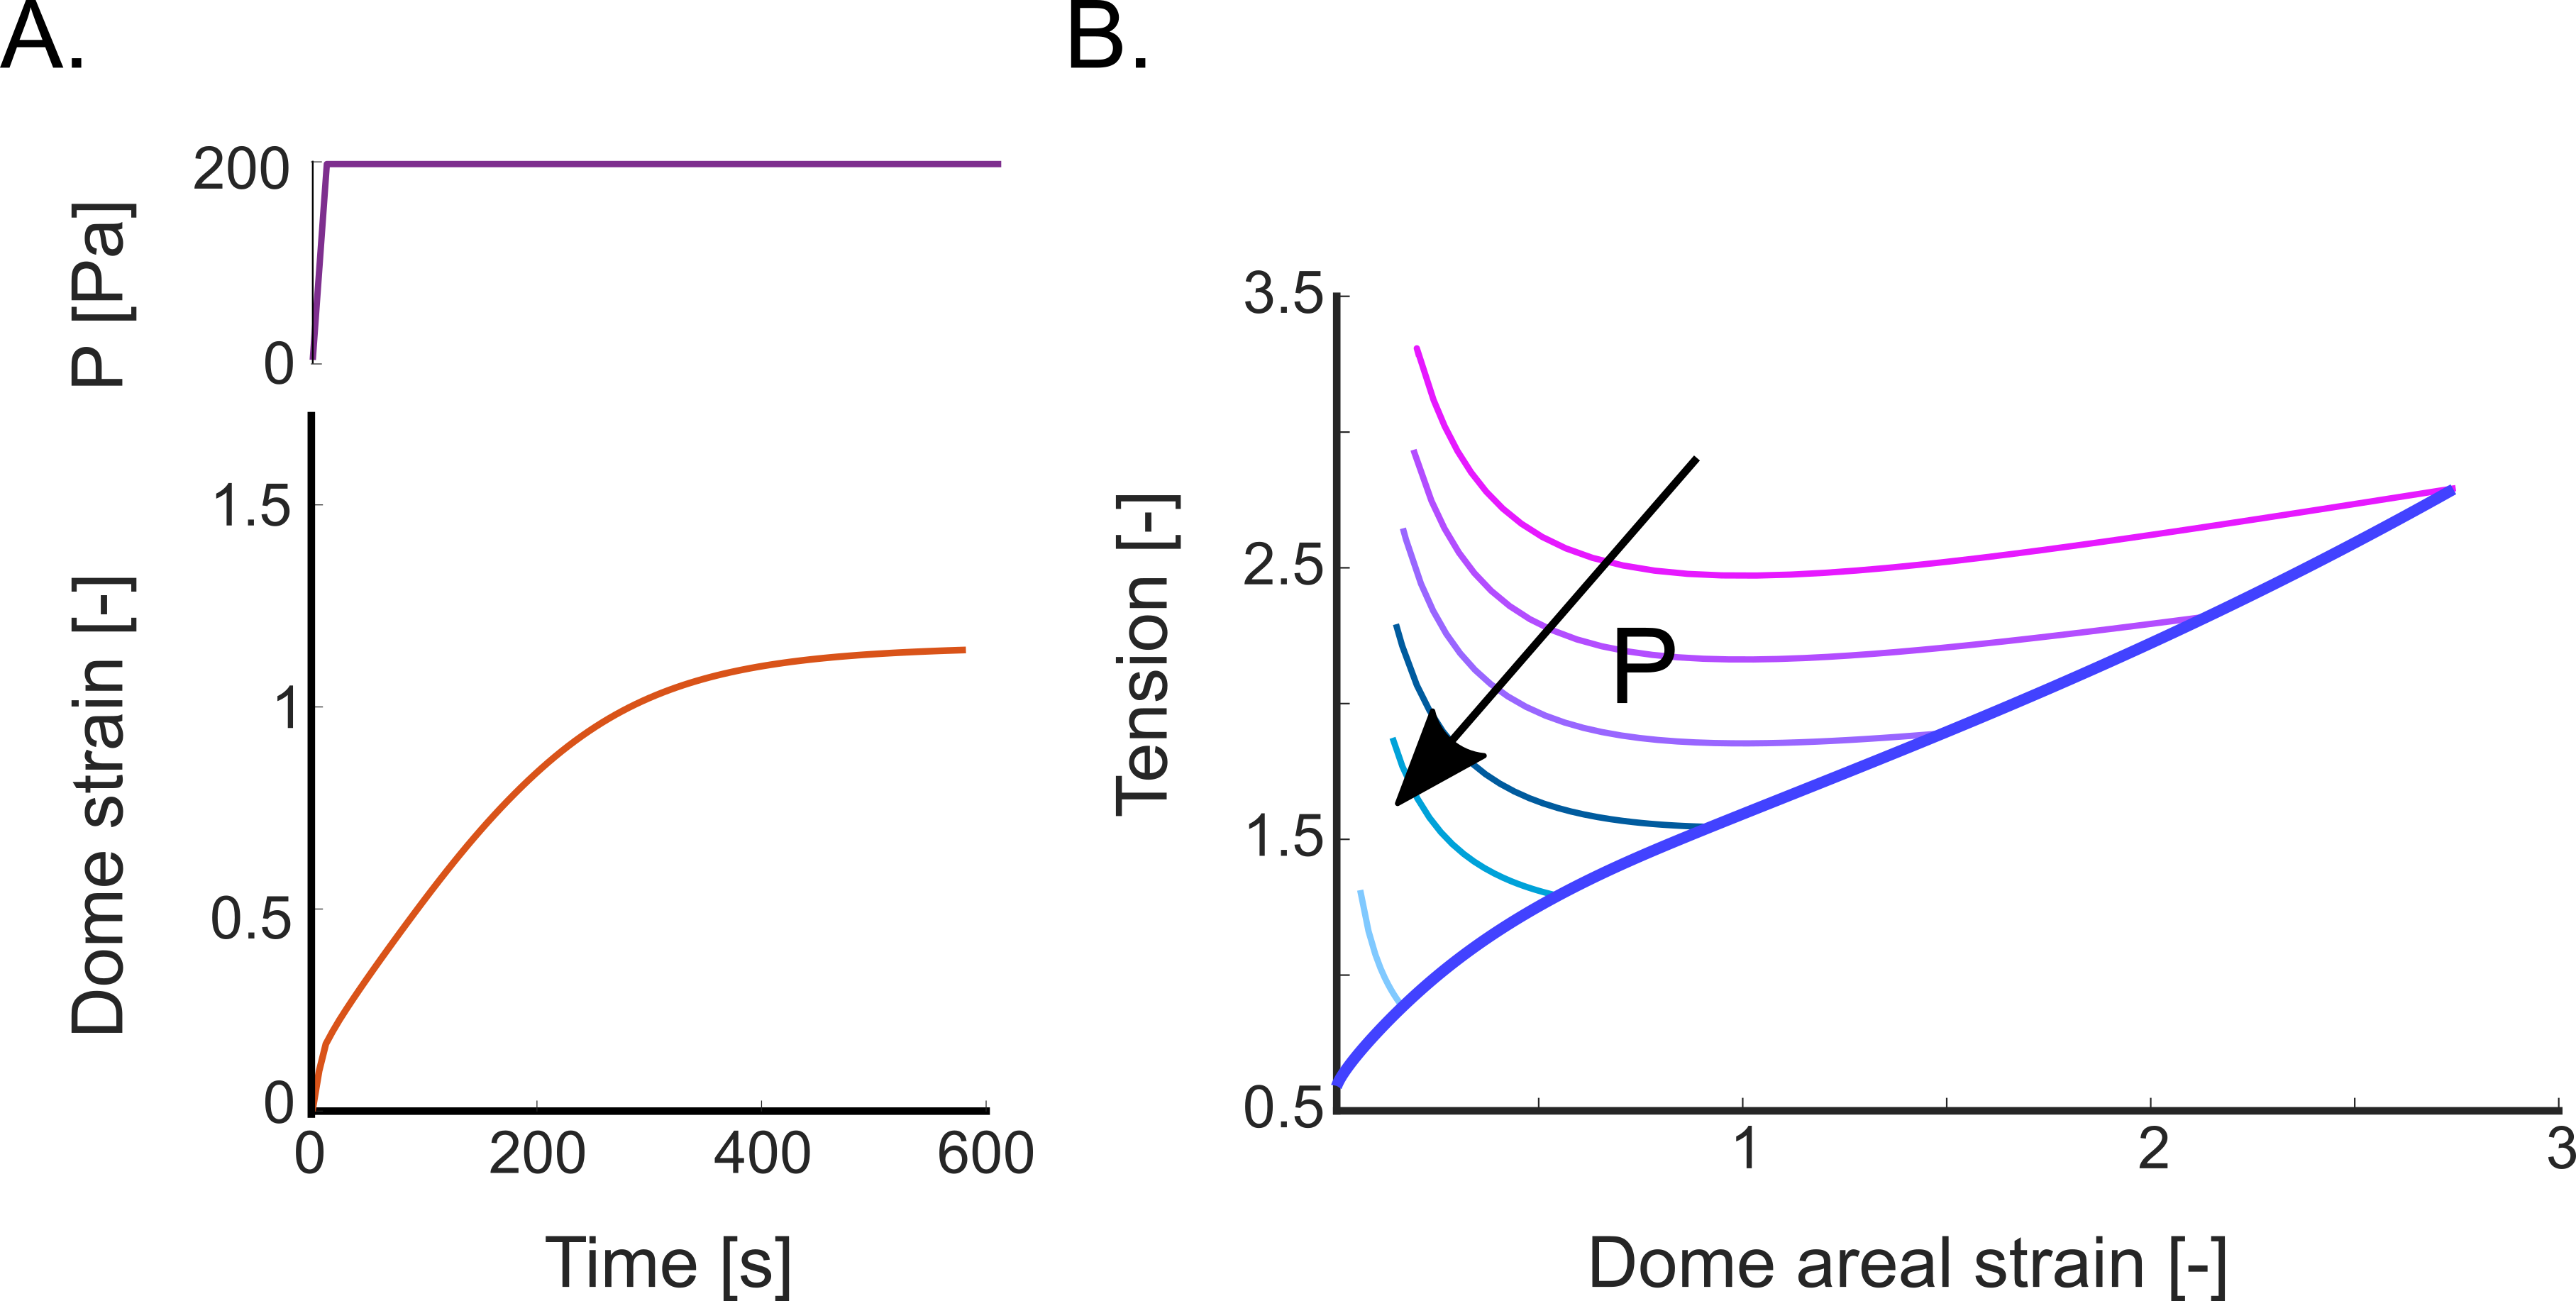
\includegraphics[width=\textwidth]{chap7_constitutivelawtwin.png}
	\caption{\label{fig_7_7} \textbf{Material response of the digital domes}: (A) When subjected to constant pressure, as in experiments, the digital dome inflated and reached a steady state. (B) These simulations also produced non-monotonic tension strain curves for different pressures, all leading to a steady state. Furthermore, subjecting it to a quasi-static increase in pressure produced a constitutive law (Navy blue curve) that can be mapped onto the locus of steady-state points. Tension reported here is non dimensional quantity.}
\end{figure}

The effect of the remodeling timescale is especially noticeable in cyclic stretching experiments. When digital domes are subjected to a cyclic pressure at rates that are slower than cortical dynamics, the deformations of the cells occur with the cortex being in a state close to steady state. The stored elastic energy is dissipated as the strain increases, and the cortical thickness does not change significantly. We observed that the resting area in the digital dome almost overlapped with the actual area (Figure \ref{fig_7_7} B bottom). This slow rate of 0.2 Pa/s provides cells with sufficient time to remodel and dissipate viscoelastic stresses. Viscoelastic and turnover timescales in simulations are around 10-30s, which means that over a period of 2000s, the dome stretches to considerably large strains of 250-300\% and returns to its original flat state.

In contrast, when cells in a dome are subjected to cyclic pressure at rates faster than cortical dynamics, they accumulate strains due to insufficient time to dissipate viscoelastic stress. In this case, the actual area changes more rapidly than the viscoelastic and turnover timescales permit (Figure \ref{fig_7_7} B top). Consequently, along with the change in the actual area, the resting area also changes, but at a slower pace. During deflation, the resting area decreases but cannot decrease completely before the next inflation cycle begins, causing the tissue to stretch further. Eventually, a limit cycle is reached, wherein cells stably oscillate between two strains, and the resting area oscillates as well, but at a smaller amplitude (Figure \ref{fig_7_7} B top).


\begin{figure}
	\centering
	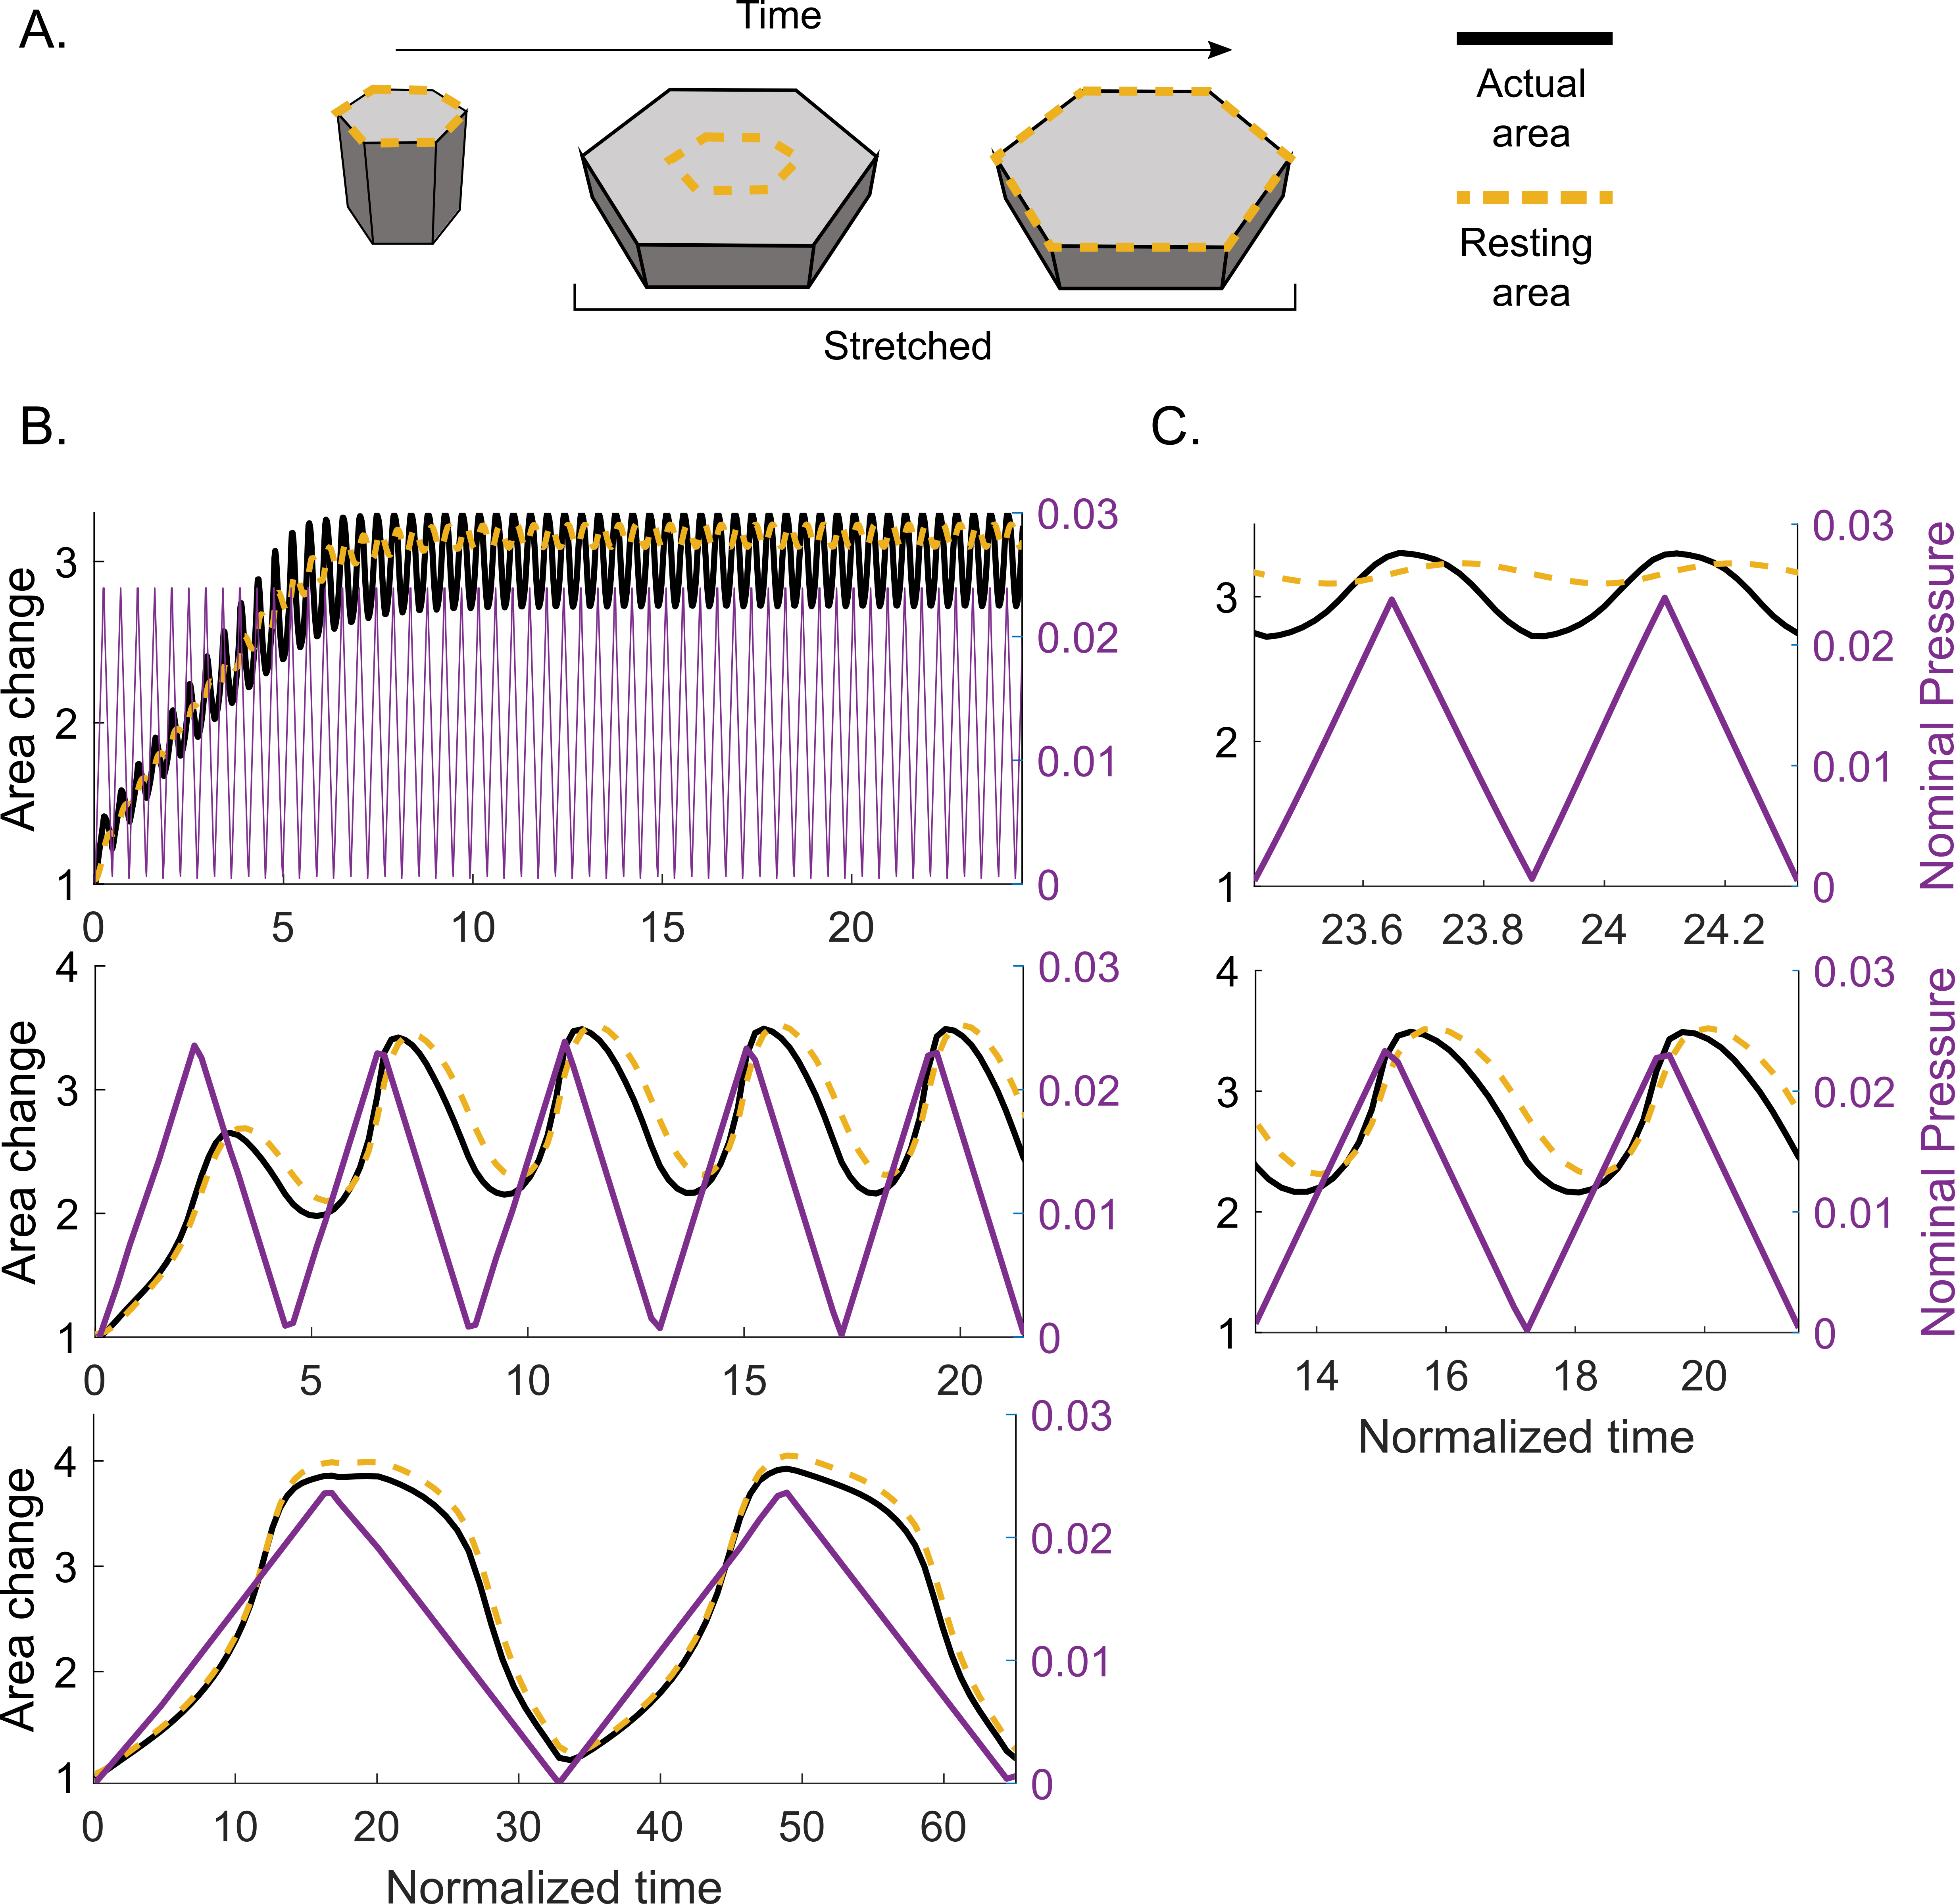
\includegraphics[width=\textwidth]{chap7_area.png}
	\caption{\label{fig_7_8} \textbf{Evolution of Resting and Actual Cell Areas in Response to Cyclic Pressure}: (A) Illustration of resting and actual cell areas in a monolayer during stretching. (B) Fold area change relative to the initial area, with three rows of panels showing the evolution of area change over normalized time. Digital domes were subjected to cycles with three different time intervals: 20s (top), 266s (middle), and 2000s (bottom). (C) Inset of the last two cycles in the case of fast and moderate rates.
	}
\end{figure}

To sum up, the active gel model explains the material response of epithelial tissue depending on the rate at which pressure is applied. The concept of resting area enables us to understand that slower rates allow for cell remodeling and dissipation of viscoelastic stress, while faster rates result in strain accumulation due to insufficient time for dissipation. This active viscoelastic behavior is the outcome of timescales associated with cortical remodeling.

\clearpage
\hypertarget{summary}{%
	\section{Summary and Discussion}\label{summary}}

In this chapter, we investigated the mechanics of epithelial tissue by applying pressure at varying rates. Initially, we applied a constant pressure of 200Pa, which led to the dynamic inflation of domes and eventually reached a steady state in strain. Due to the spherical geometry of the tissue and Laplace’s law, we observed a non-monotonous tension-strain curve in response to the constant pressure. We found that the true tension-strain curve exhibited increasing tension with respect to strains at lower values, but at higher strains, the tension appeared to be independent of the strains. 

Furthermore, our measurements showed that the domes accumulated strain through the cycles when probed with fast-changing pressure and reached a steady-state in later cycles. However, when stretched slowly, the domes reached higher strains without accumulating strain at the end of the cycle. To understand the behavior of epithelial tissue, we used the computational framework developed by Adam Ouzeri and Marino Arroyo, which shows that the mechanical response of the domes to pressure is dependent on active viscoelasticity \cite{ouzeri2023}. The digital dome studies highlighted the interplay of different timescales, which are the reflection of the interaction between cortical turnover, crosslinker dynamics, and network reorganization, allowing for large deformations and rapid shape changes. 

Our results can be interpreted using a multidimensional Maxwell model. The classical Maxwell model consists of a spring and a dashpot, which represent the elastic and viscous elements, respectively. In our case, we can imagine a similar model with two branches: one branch includes a spring and a dashpot to represent the passive viscoelasticity, and a second branch includes an active spring to represent the active component  (see fig \ref{fig_7_9}). The active spring is always present, but if the system is stretched at slower rates, the dashpot drives the dominant mechanical response. Conversely, if stretched at faster rates, the elastic spring deformation dominates. By separating the passive and active components, we can better understand how each contributes to the overall viscoelastic behavior and associated timescales. 

\begin{figure}[b!]
	\centering
	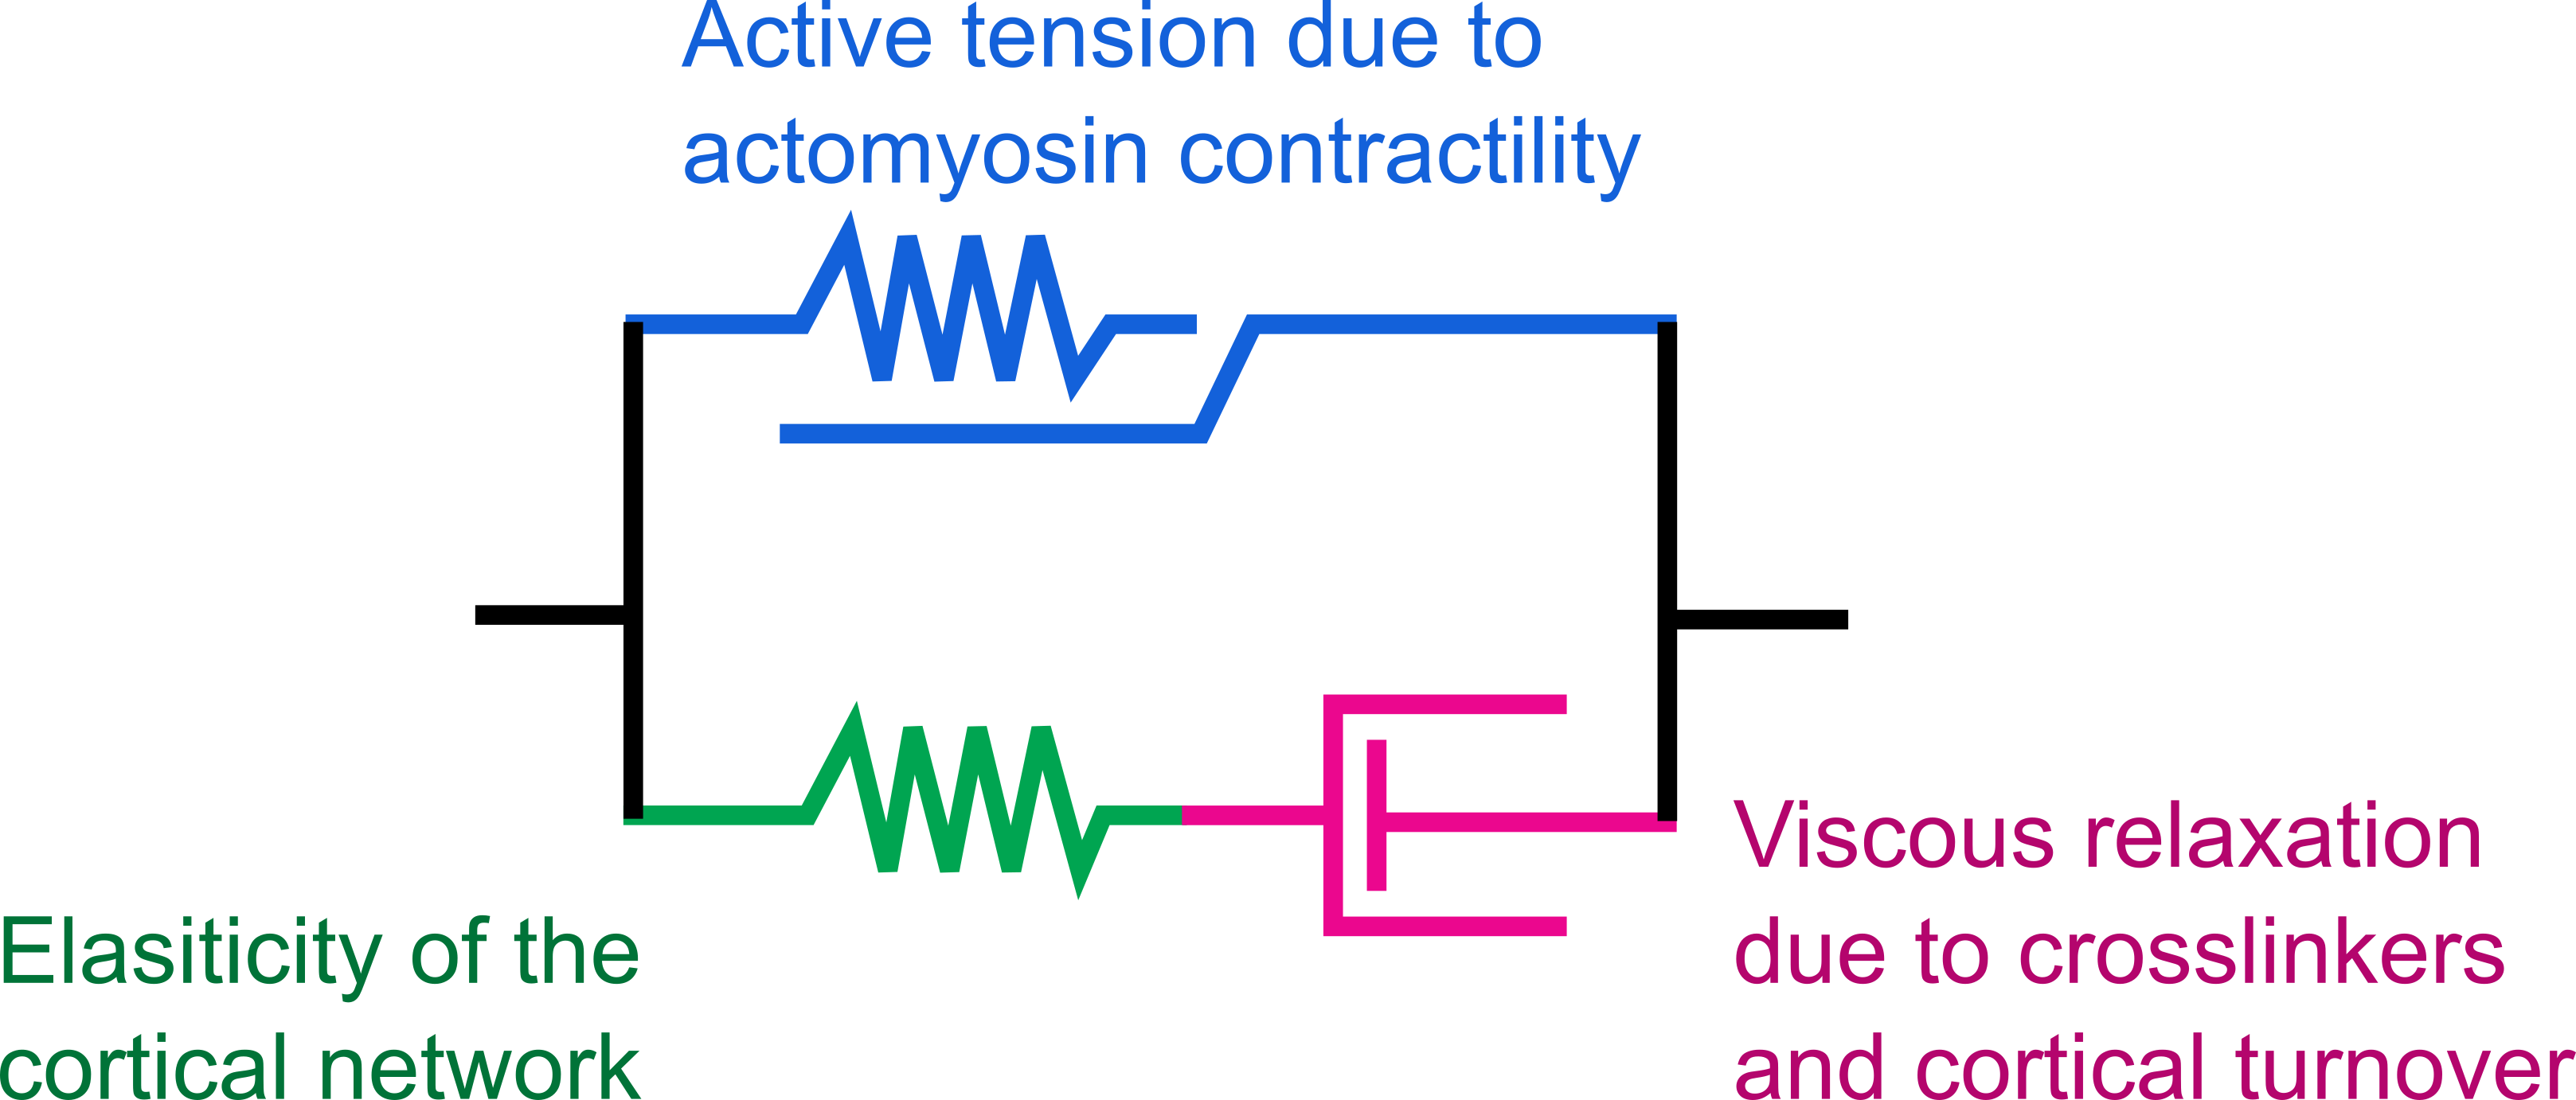
\includegraphics[width=0.75\textwidth]{chap7_maxwell.png}
	\caption{\label{fig_7_9} \textbf{Representational viscoelasticity model}: The model can be understood using a spring and dashpot analogy with two branches: The first branch is an active spring representing the contractile forces applied by the actomyosin cortex. The second branch has two components, one for the elasticity of the network and the second for the viscous relaxation that occurs due to turnover of the network.
	}
\end{figure}

Previous research has approached the system in a similar manner, where epithelial tissue was modeled using viscoelastic models of springs and dashpots. One particularly interesting model was developed by Khalilgharibi et. al., which characterizes the response of a suspended monolayer to stretch and demonstrates that the dynamics are similar to that of a single cell, due to the role of the actomyosin cortex 
\cite{khalilgharibi2019}. They used a model with two springs in parallel, one of which can change its resting length dynamically. The model explains the relaxation of the monolayer, as the active contractility of the cortex changes the resting length of the active spring, which closely relates to our "resting area" concept. 

Another study by Clément et al. (2017) found that viscoelastic dissipation could explain the shortening or elongation of cell junctions in Drosophila embryos \cite{clement2017}. They demonstrated that the dissipation occurs at the minute timescale, which coincides with myosin pulses, and that actin turnover plays a key role in this dissipation. These pulses have a ratchet-like mechanical effect that drives junction shortening and causes tissue folding. This ratcheting effect is reminiscent of the cyclic stretching at faster rates, where cells stretch more and more every cycle. Similar to the authors of the study, we explain the strain accumulation by incomplete dissipation of viscoelastic stress due to deformation faster than the remodeling timescale.

In this chapter, we have established a connection between the dynamic material response of epithelial tissue and active viscoelasticity using a computational model. We employed a theoretical framework that explains the time-dependent mechanics of tissues, observed in experiments, in terms of the remodeling timescales of molecular components.

Regarding molecular components, although we did not use pharmacological treatments, the MOLI system can accommodate the introduction of drugs. Various components in the actin network enable cortical tension modulation through pharmacological interventions that target specific molecular targets \cite{cartagena-rivera2016}. For instance, Latrunculin depolymerizes the actin network, while Blebbistatin decreases cortical tension by inhibiting myosin activity. Conversely, Calyculin-A enhances contractility by accelerating Myosin II phosphorylation. In future experiments, these pharmacological interventions could be employed to identify the molecular pathways involved in the tissue's mechanical response.

Our experimental system focused on probing the response of suspended tissues at short timescales (minutes), which correspond to the timescale of acto-myosin network remodeling. We did not observe any cellular rearrangement, extrusion, or division at this timescale in our system, except for rare exceptions. Long-term experiments were not performed, as they were outside the scope of this study due to the suspected involvement of other cytoskeletal components, such as intermediate filaments. Latorre et al. (2018) observed the activation of intermediate filaments in extremely stretched cells (>300\%) and proposed that this caused re-stiffening, preventing the cells from stretching excessively \cite{latorre2018}. This observation motivated the strain-limiting mechanism imposed in our model.

Latorre et al. also demonstrated heterogeneity in cell stretching, along with active superelasticity. However, in our experiments, we did not observe the coexistence of stretched and super-stretched cells. This might be due to the relatively shorter timescales in our experiments compared to long-term quasi-static deformation of spontaneous domes.

A recently published study \cite{duque2023} shows that strain stiffening is dependent on the strain and strain rates. The tissue stiffens at higher strains, but for higher strain rates, the stiffening is more pronounced at higher strains (15\%) than lower strains (120\%). They demonstrated that this response is due to the supracellular network of intermediate filaments. In our experiments, we could only control pressure and pressure rates. However, if needed, we can track the strains and quantify strain rates to explore the mechanics. When plotting tension-strain curves for different pressure rates, we noticed characteristics of stiffening at higher strains and higher rates. In the model, there is no rate-dependent strain stiffening. In the future, we could easily incorporate this aspect into the model.

By combining the model and experiments, we understand that the epithelium behaves as an active viscoelastic material. In the next chapter, we will endeavor to harness this knowledge of active viscoelasticity to generate transformations of domes into various structures.
